\chapter{Theoretical Background}

A sophisticated globe rendering system needs to rely on some mathematical foundations. These foundations together with different theories and algorithms developed for globe rendering works as a base for the research of this thesis.

\section{Modelling Globes}

We will discuss different proposed methods used for modelling and rendering of globes. The globe can be modelled either as a sphere or an ellipsoid and there are different tessellation schemes for meshing the globe. Different map projections can also be considered and it all ties together with a choice of level of detail algorithm.

\subsection{Globes as Ellipsoids}

Planets, moons and asteroids are generally more accurately modelled as ellipsoids than as spheres. Planets are often stretched out along their equatorial axes due to their rotation which causes the centripetal force to counter some of the gravitational force acting on the mass. This effect was proven in 1687 by Isac Newton in Principia Mathematica \cite{newton87}. The rotation causes a self-gravitating fluid body in equilibrium to take the form of an oblate ellipsoid, otherwise known as a biaxial ellipsoid with one semimajor and one semiminor axis. Globes can be modeled as triaxial ellipsoids for more accuracy when it comes to smaller, more irregularly shaped objects. For example Phobos, one of Mars's two moons, is more accurately modeled as a triaxial ellipsoid with radii of $27 \times 22 \times 18$ km \cite{cozzi11}.

The World Geodetic System 1984 (WGS84) standard defined by National Geospatial-Intelligence Agency (NGA) models the Earth as a biaxial ellipsoid with a semimajor axis of 6,378,137 m and a semiminor axis of 6,356,752.3142 m \cite{cozzi11}. This is what is known as a reference ellipsoid; a mathematical description that approximates the geoid of the earth as closely as possible. The WGS84 standard is widely used for GIS and plays an important role in accurate placements of objects such as satellites or spacecrafts with position coordinates relatively close to the Earth's surface. In the WGS84 coordinate system, the x-axis points to the prime meridian, the z-axis points to the north pole and the y-axis completes the right handed coordinate system, see figure \ref{fig:wgs84}.

\begin{figure}
\centering
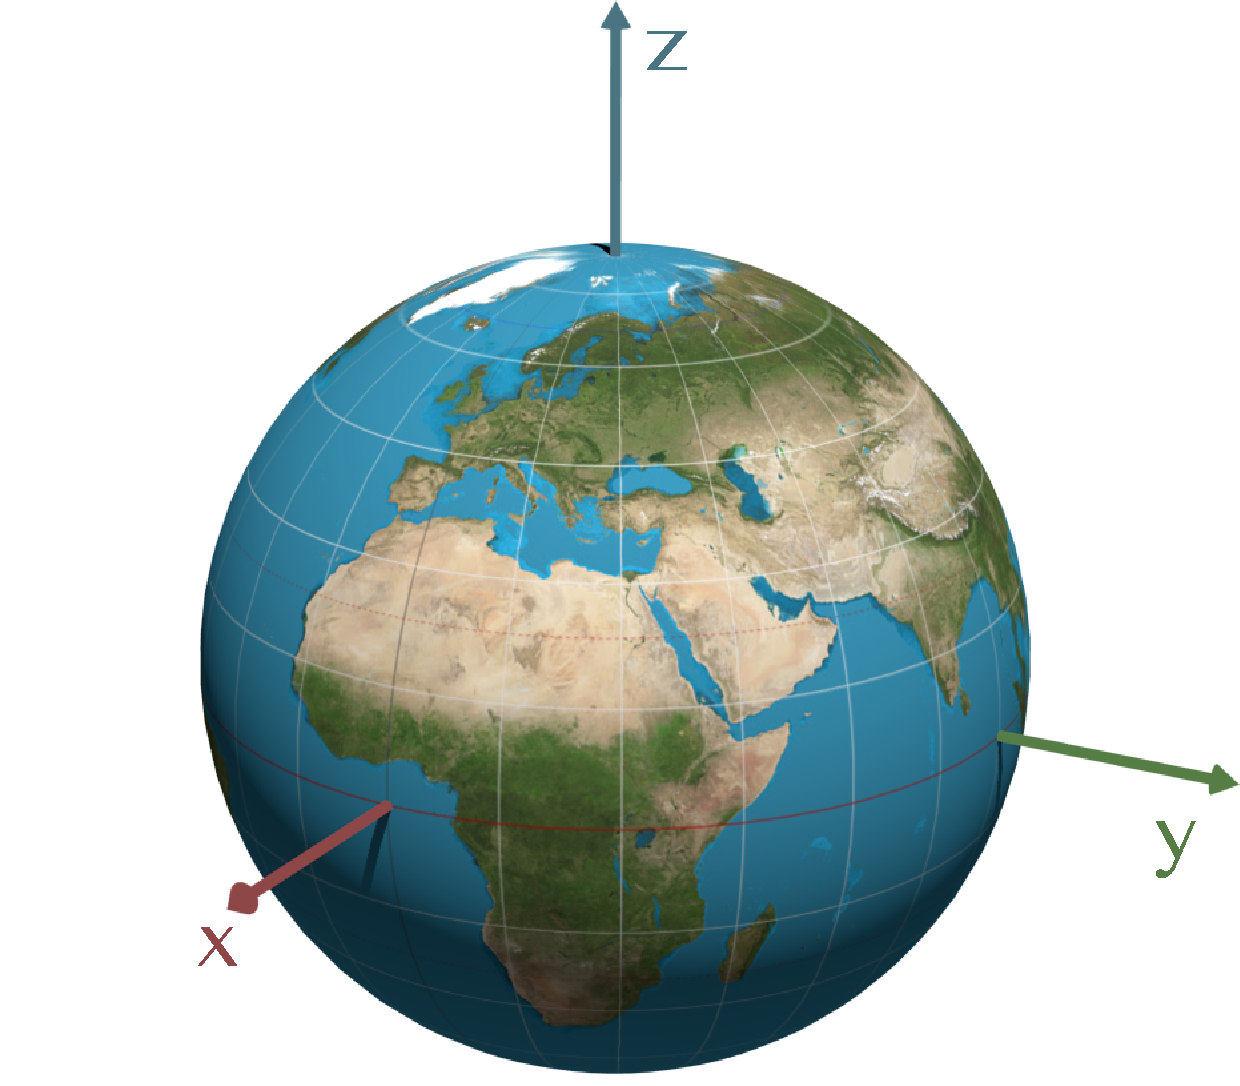
\includegraphics[scale=0.25]{figures/wgs84.pdf}
\caption{The WGS84 coordinate system and globe.}
\label{fig:wgs84}
\end{figure}

\subsection{Tesselating the Ellipsoid}

Triangle models are still the most common way of modeling renderable objects in 3D computer graphics softwares, even though other rendering techniques such as volumetric ray casting also can be considered for terrain rendering \cite{cozzi11}.

A triangle mesh, or more generally a polygon mesh, is defined by a limited number of surface elements. This means that ellipsoids need to be approximated by some sort of tessellation or subdivision surface when modeled as a polygon mesh. There are several techniques for tessellating an ellipsoid. Some of them are covered in this section.

\subsubsection{Geographic Grid Tessellation}
\label{sec:geogrid}
Tessellating the ellipsoid using a geographic grid is a very straightforward approach. Ellipsoid vertex positions can be calculated using a transform from geographic coordinates to cartesian model space coordinates \cite[p. 25]{cozzi11}. Figure \ref{fig:tesselation_geo} shows three geographic grid tessellations of ellipsoids with constant number of latitudinal segments of 4, 8 and 16 respectively.

A common issue with geographic grids is something referred to as polar pinching. At both of the poles, segments will be pinched to one point which leads to an increasing amount of segments per area. This in turn results in oversampling in textures as well as possible visual artefacts in shading due to the very thin quads at the poles as well as possible performance penalties for highly tessellated globes.

\begin{figure}
    \centering
    \begin{subfigure}[b]{0.2\textwidth}
        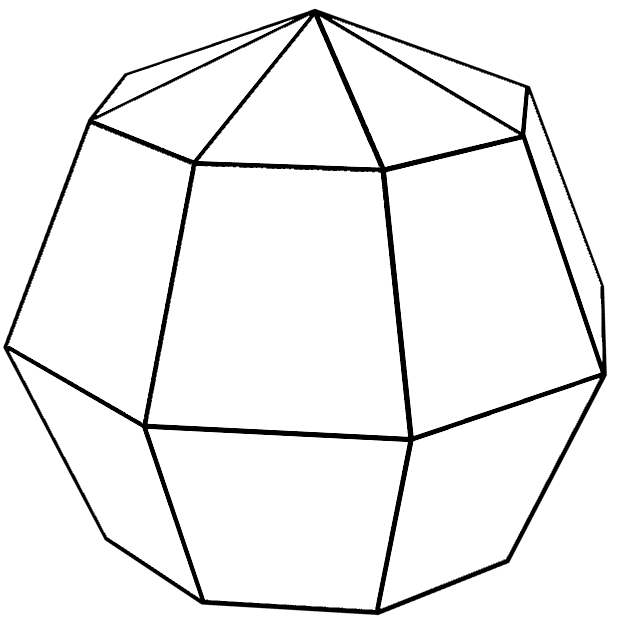
\includegraphics[width=\textwidth]{figures/tessellation/tessellation_geo1.png}
    \end{subfigure}
    ~ %add desired spacing between images, e. g. ~, \quad, \qquad, \hfill etc. 
      %(or a blank line to force the subfigure onto a new line)
    \begin{subfigure}[b]{0.2\textwidth}
        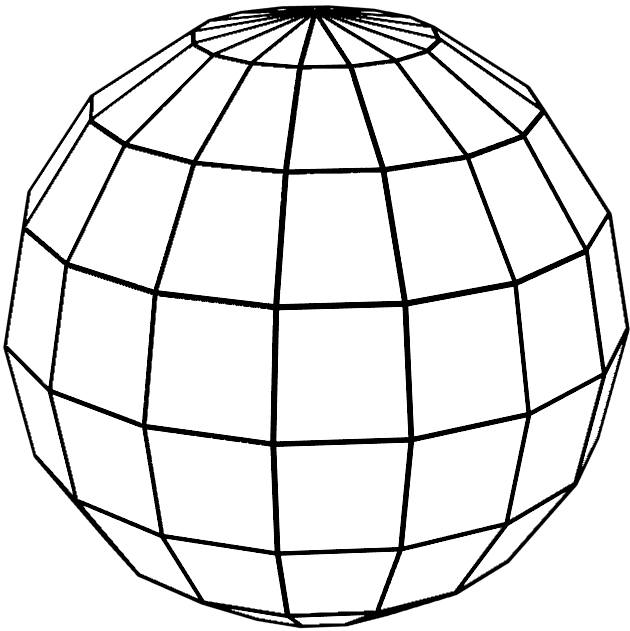
\includegraphics[width=\textwidth]{figures/tessellation/tessellation_geo2.png}
    \end{subfigure}
    ~ %add desired spacing between images, e. g. ~, \quad, \qquad, \hfill etc. 
    %(or a blank line to force the subfigure onto a new line)
    \begin{subfigure}[b]{0.2\textwidth}
        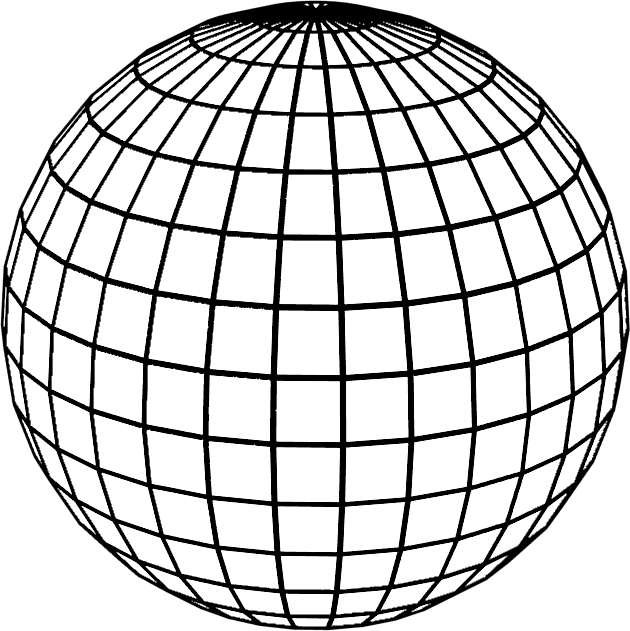
\includegraphics[width=\textwidth]{figures/tessellation/tessellation_geo3.png}
    \end{subfigure}
    \caption{Geographic grid tesselation.}
    \label{fig:tesselation_geo}
\end{figure}

\subsubsection{Quadrilateralized Spherical Cube Tessellation}
 
Another common tessellation method for spheres which can be generalized to ellipsoids is the quadrilateralized spherical cube tessellation. The standard approach is to subdivide a cube centered in the origin and then normalize the coordinates of all vertices to map them on a sphere. There are also other more complicated schemes designed to work with specific map projections \cite{dimi15}.

To model an ellipsoid from a sphere, the vertices can be linearly transformed with a scaling in the $x$, $y$, and $z$ directions individually. Figure \ref{fig:tesselation_cube} shows a tessellated spherical cube of four different detail levels.

\begin{figure}
    \centering
    \begin{subfigure}[b]{0.2\textwidth}
        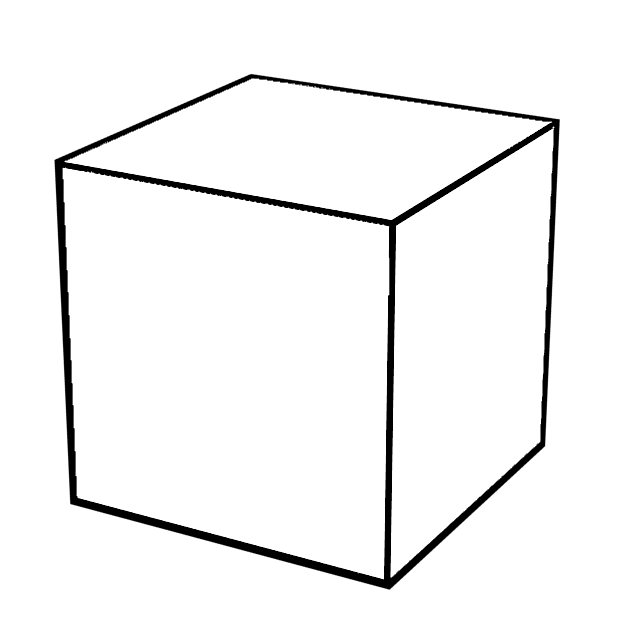
\includegraphics[width=\textwidth]{figures/tessellation/tessellation_cube1.png}
    \end{subfigure}
    ~ %add desired spacing between images, e. g. ~, \quad, \qquad, \hfill etc. 
      %(or a blank line to force the subfigure onto a new line)
    \begin{subfigure}[b]{0.2\textwidth}
        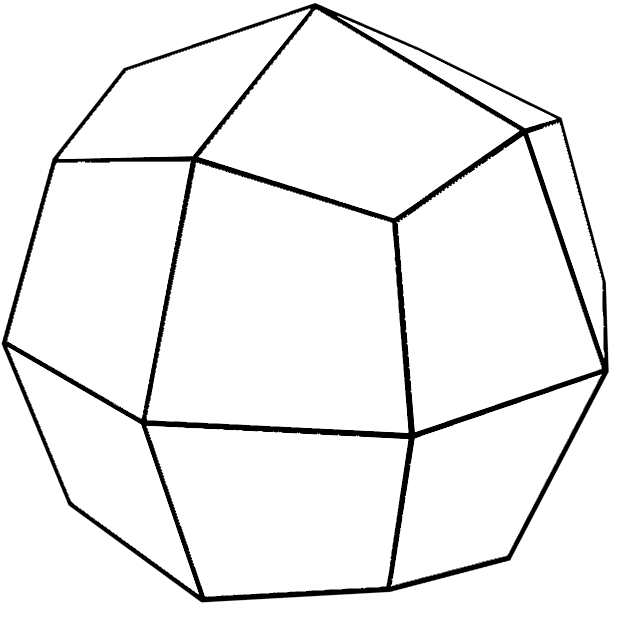
\includegraphics[width=\textwidth]{figures/tessellation/tessellation_cube2.png}
    \end{subfigure}
    ~ %add desired spacing between images, e. g. ~, \quad, \qquad, \hfill etc. 
    %(or a blank line to force the subfigure onto a new line)
    \begin{subfigure}[b]{0.2\textwidth}
        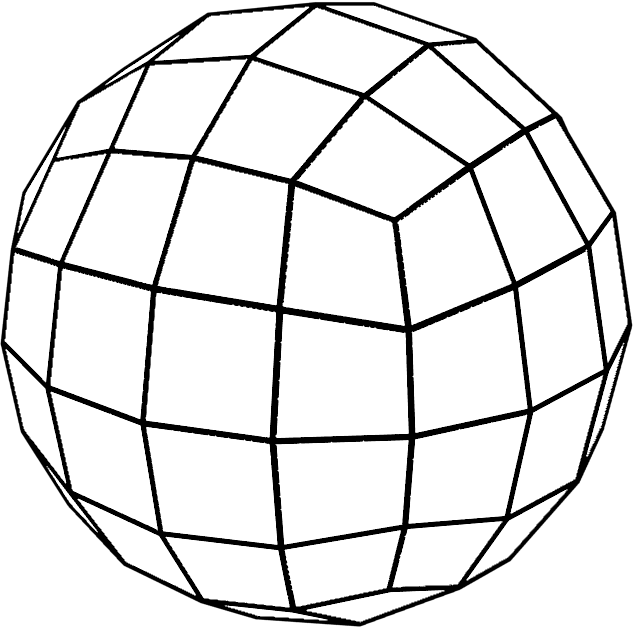
\includegraphics[width=\textwidth]{figures/tessellation/tessellation_cube3.png}
    \end{subfigure}
    ~ %add desired spacing between images, e. g. ~, \quad, \qquad, \hfill etc. 
    %(or a blank line to force the subfigure onto a new line)
    \begin{subfigure}[b]{0.2\textwidth}
        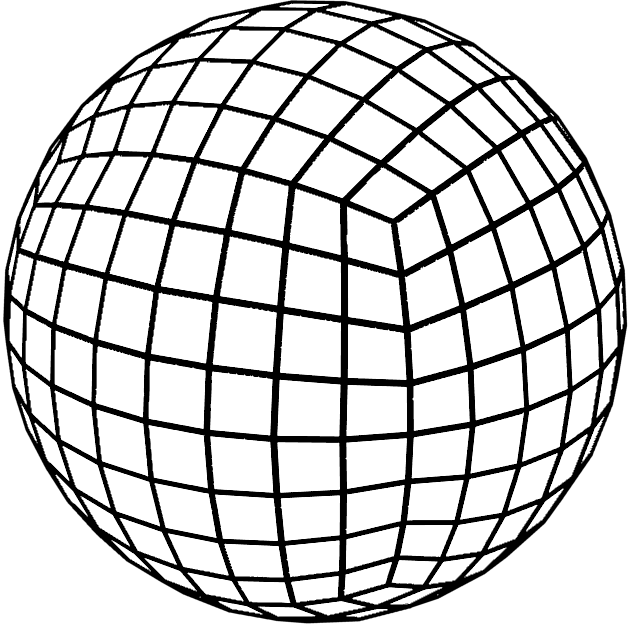
\includegraphics[width=\textwidth]{figures/tessellation/tessellation_cube4.png}
    \end{subfigure}
    \caption{Quadrilateralized spherical cube tessellation.}
    \label{fig:tesselation_cube}
\end{figure}

\subsubsection{Hierarchical Triangular Mesh}

The hierarchical triangular mesh (HTM) is a method of modeling the sky dome as a sphere proposed by astronomers in the Sloan Digital Sky Survey \cite{htm}. Instead of uniformly dividing cube faces, an alternative option is to subdivide a normalized octahedron by, in each subdivision step, split every triangle into four new triangles, see figure \ref{fig:tesselation_htm}. An ellipsoid can be created from the sphere by normalizing the coordinates and linearly rescaling them the same way that can be done for the spherical cube tessellation.

\begin{figure}
    \centering
    \begin{subfigure}[b]{0.2\textwidth}
        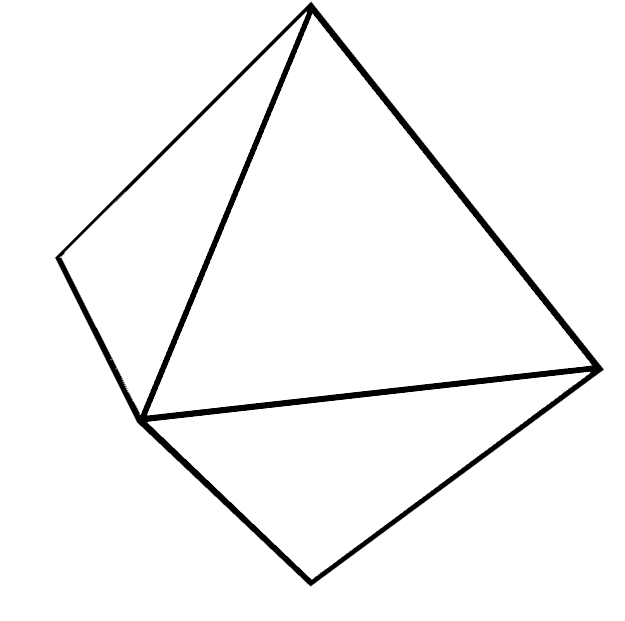
\includegraphics[width=\textwidth]{figures/tessellation/tessellation_htm1.png}
    \end{subfigure}
    ~ %add desired spacing between images, e. g. ~, \quad, \qquad, \hfill etc. 
      %(or a blank line to force the subfigure onto a new line)
    \begin{subfigure}[b]{0.2\textwidth}
        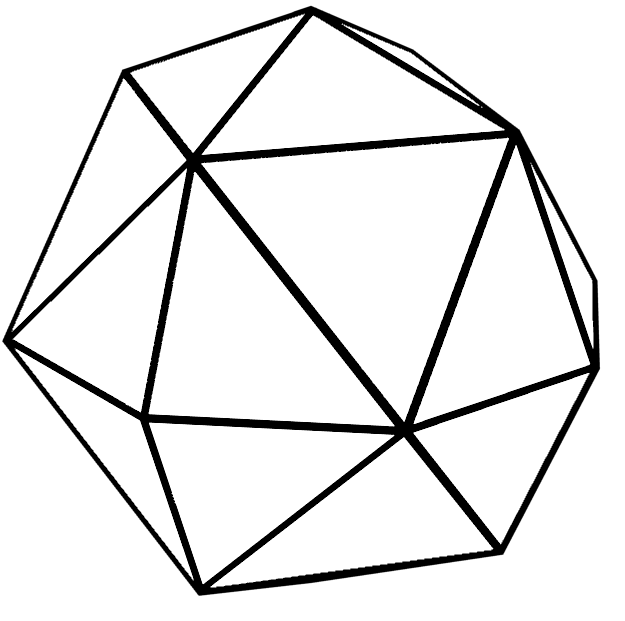
\includegraphics[width=\textwidth]{figures/tessellation/tessellation_htm2.png}
    \end{subfigure}
    ~ %add desired spacing between images, e. g. ~, \quad, \qquad, \hfill etc. 
    %(or a blank line to force the subfigure onto a new line)
    \begin{subfigure}[b]{0.2\textwidth}
        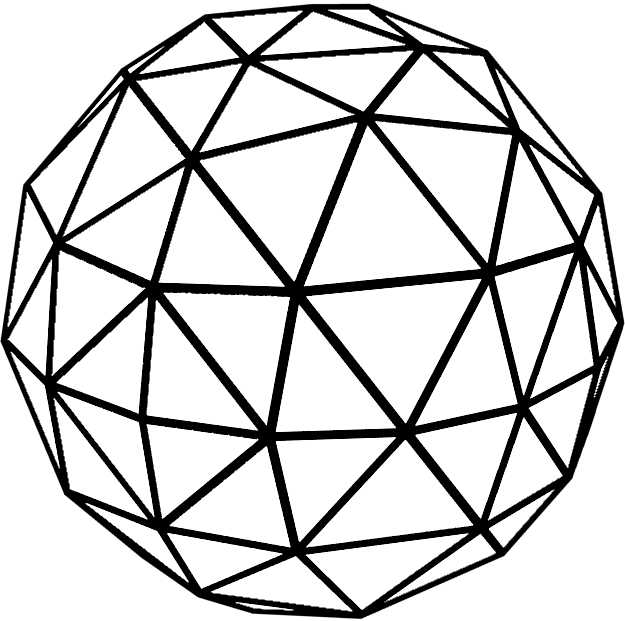
\includegraphics[width=\textwidth]{figures/tessellation/tessellation_htm3.png}
    \end{subfigure}
    ~ %add desired spacing between images, e. g. ~, \quad, \qquad, \hfill etc. 
    %(or a blank line to force the subfigure onto a new line)
    \begin{subfigure}[b]{0.2\textwidth}
        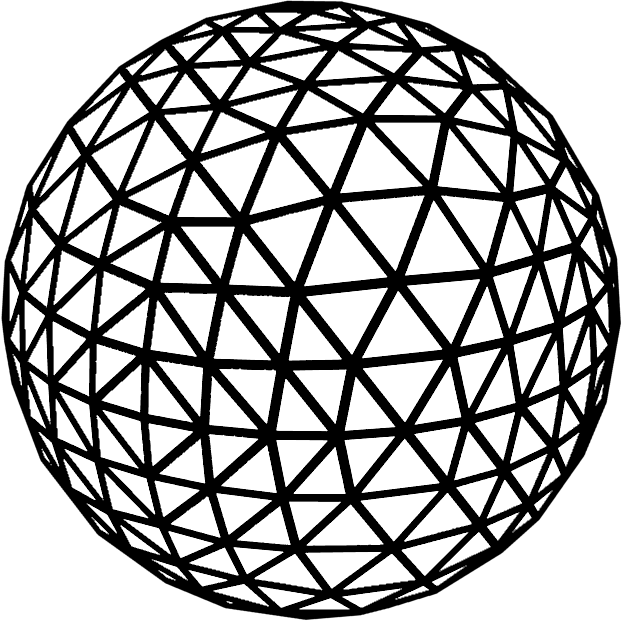
\includegraphics[width=\textwidth]{figures/tessellation/tessellation_htm4.png}
    \end{subfigure}
    \caption{Hierarchical triangular mesh tesselation.}
    \label{fig:tesselation_htm}
\end{figure}

\subsubsection{Hierarchical Equal Area IsoLatitude Pixelation}

Hierarchical Equal Area IsoLatitude Pixelation (HEALPix) is spherical tessellation scheme with corresponding map projection. The base level of the tessellation is built up of twelve quads, similar to a rhombic dodecahedron, which each can be subdivided further. The tessellation in figure \ref{fig:tesselation_healpix} shows how the vertices in the HEALPix tessellation leads to curvilinear quads.

\begin{figure}
    \centering
    \begin{subfigure}[b]{0.2\textwidth}
        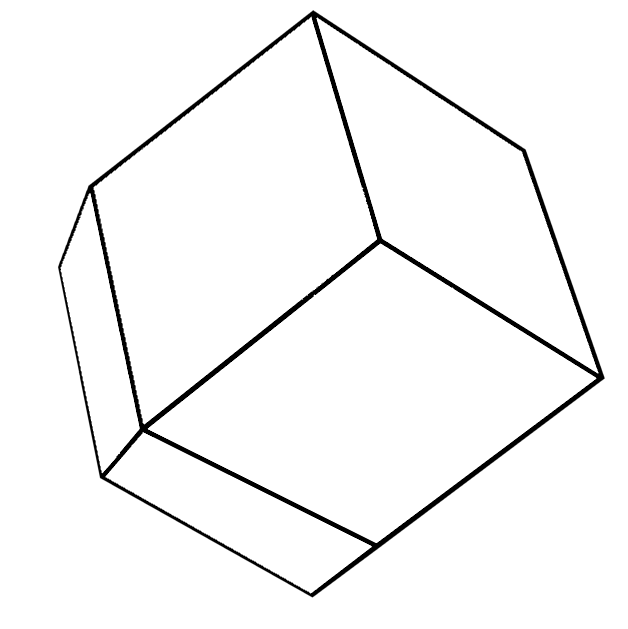
\includegraphics[width=\textwidth]{figures/tessellation/tessellation_healpix1.png}
    \end{subfigure}
    ~ %add desired spacing between images, e. g. ~, \quad, \qquad, \hfill etc. 
      %(or a blank line to force the subfigure onto a new line)
    \begin{subfigure}[b]{0.2\textwidth}
        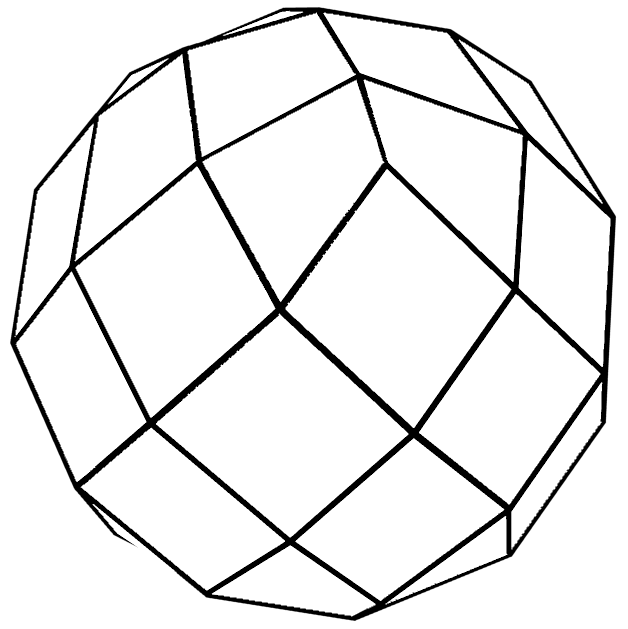
\includegraphics[width=\textwidth]{figures/tessellation/tessellation_healpix2.png}
    \end{subfigure}
    ~ %add desired spacing between images, e. g. ~, \quad, \qquad, \hfill etc. 
    %(or a blank line to force the subfigure onto a new line)
    \begin{subfigure}[b]{0.2\textwidth}
        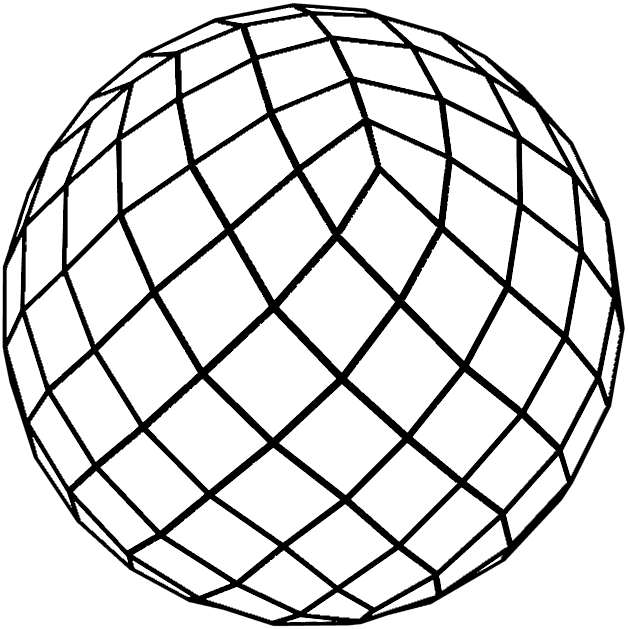
\includegraphics[width=\textwidth]{figures/tessellation/tessellation_healpix3.png}
    \end{subfigure}
    \caption{HEALPix tesselation.}
    \label{fig:tesselation_healpix}
\end{figure}

\subsubsection{Geographic Grid Tessellation With Polar Caps}

In their description of the ellipsoidal clipmaps method, Dimitrijevi\'{c} and Ran\v{c}i\'{c} introduces polar caps to avoid polar issues related to geographic grids \cite{dimi15}. The polar caps are simply used as a replacement of the problematic, oversampled regions around the poles. The caps can be modelled as grids projected onto the ellipsoid surface in their own georeferenced coordinate systems. One obvious issue with polar caps is the edge problem that occurs due to the fact that the caps are defined as separate meshes with vertices that do not coincide with the geographic vertices of the equatorial region, see figure caps. Dimitrijevi\'{c} and Ran\v{c}i\'{c} solves the issue by using a type of edge blending between the equatorial and polar segments \cite{dimi15}. Figure \ref{fig:tesselation_caps} shows a sphere tessellated with one equatorial region and two polar regions.

\begin{figure}
    \centering
    \begin{subfigure}[b]{0.2\textwidth}
        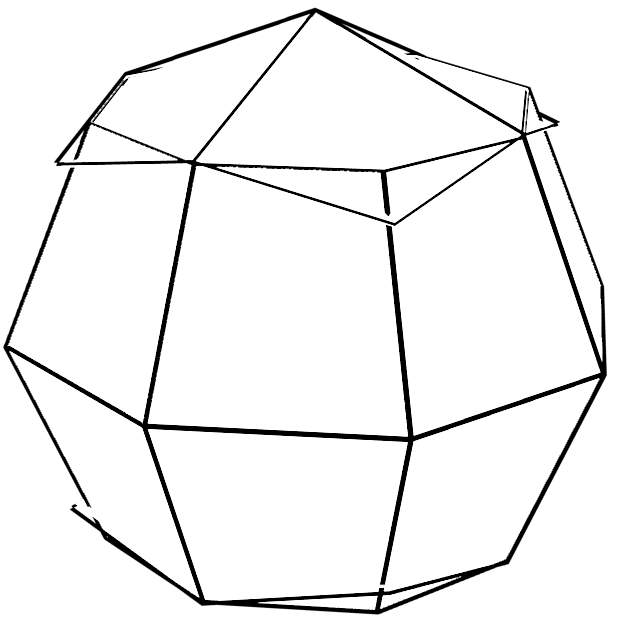
\includegraphics[width=\textwidth]{figures/tessellation/tessellation_caps_proj1.png}
    \end{subfigure}
    ~ %add desired spacing between images, e. g. ~, \quad, \qquad, \hfill etc. 
      %(or a blank line to force the subfigure onto a new line)
    \begin{subfigure}[b]{0.2\textwidth}
        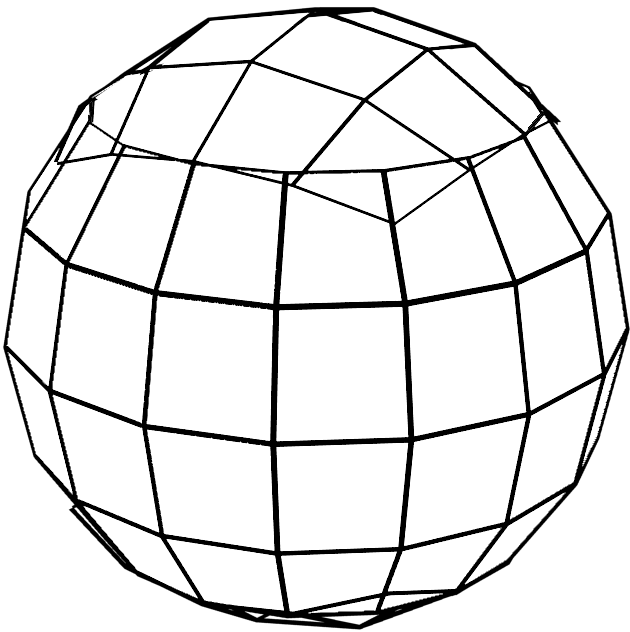
\includegraphics[width=\textwidth]{figures/tessellation/tessellation_caps_proj2.png}
    \end{subfigure}
    ~ %add desired spacing between images, e. g. ~, \quad, \qquad, \hfill etc. 
    %(or a blank line to force the subfigure onto a new line)
    \begin{subfigure}[b]{0.2\textwidth}
        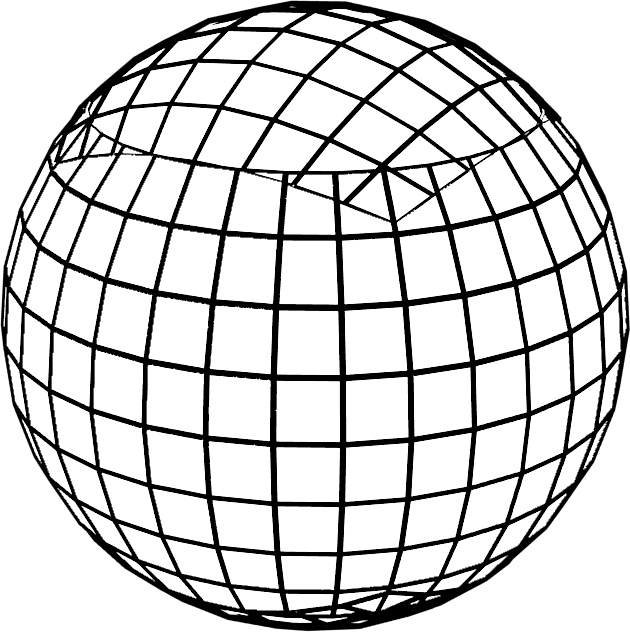
\includegraphics[width=\textwidth]{figures/tessellation/tessellation_caps_proj3.png}
    \end{subfigure}
    \caption{Geographic tessellation of an ellipsoid with polar caps.}
    \label{fig:tesselation_caps}
\end{figure}

\subsection{2D Parameterisation for Map Projections}

A map projection $P$ defines a transformation from cartesian model space coordinates to georeferenced (projected) coordinates, as in equation \ref{eq:proj}. The inverse projection $P^{-1}$ is used to find positions on the globe surface in model space given georeferenced coordinates as in equation \ref{eq:invproj}.

\begin{equation}
\label{eq:proj}
\begin{pmatrix} s  \\ t  \end{pmatrix}_{ georeferenced }=\vec { P } (x,y,z),
\end{equation}

\begin{equation}
\label{eq:invproj}
\begin{pmatrix} x \\ y \\ z \end{pmatrix}_{ modelspace }=\vec { P }^{-1} (s ,t ),
\end{equation}

Where $(x,y,z)^T$ is the cartesian coordinates of a point on the ellipsoid surface. The parameters $s$ and $t$ are georeferenced coordinates defining all positions on the globe. The georeferenced coordinates can have different definition range depending on which projection is used.

The globally positive gaussian curvature of any ellipsoid makes it impossible to unproject it on a flat 2D surface without any distortions. Different projections are used for different purposes. Equal-area projections preserve the size of a projected area as $\partial s \partial t / \partial s_0 \partial t_0 = 1$, while conformal projections preserve the shape of projected objects as $\partial s / \partial t = 1$; $s_0$ and $t_0$ are coordinates at the center of the projection with no distortion. No global projection can be both area-preserving and conformal \cite{dimi15}.

There are several possibilities for defining a coordinate transform for map projections. A common approach is to project the ellipsoid onto another shape that allows for being flattened out without distortion, such as a cube, a cylinder or a plane. These types of shapes are known as developable shapes and have zero gaussian curvature.

The choice of map projection is tied together with the choice of ellipsoid tessellation. This is because the map often needs to be tiled up when rendering. Each tile has its local texture coordinate system which need to have a simple transform from the georeferenced coordinate system for texture sampling. If the tiles can be affinely transformed to the geo referenced coordinate system, texture sampling can be done on the fly; otherwise the geo referenced coordinates need to be reprojected which may be computationally heavy or impossible for real time applications.

The European Petroleum Survey Group (EPSG) has defined several standards for map projections of the Earth. Many of these are mentioned when discussing the different projections.

\subsubsection{Geographic Projections}

Geographic projections are widely used standards for parameterization of ellipsoids. The ellipsoid is projected onto a cylinder which is then unrolled to form the 2D plane of the projected coordinates.

Geographic coordinates are defined with a latitude $\phi$ and a longitude $\theta$ and works together with geographic tessellations of ellipsoids. A common issue with geographic projections is oversampling around the poles, as mentioned in section \ref{sec:geogrid}. At the poles, all longitudes will always map onto one point and the distortion increases with the absolute value of the latitude. Figure \ref{fig:proj_equi} shows an unprojected geographic map and how it wraps around the globe.

\begin{figure}[htbp]
    \centering
    \begin{subfigure}[bt]{0.4\textwidth}
        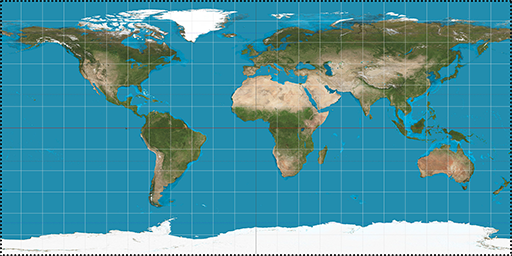
\includegraphics[width=\textwidth]{figures/developable_projected/equirectangular.png}
    \end{subfigure}
    \qquad
    \begin{subfigure}[bt]{0.15\textwidth}
        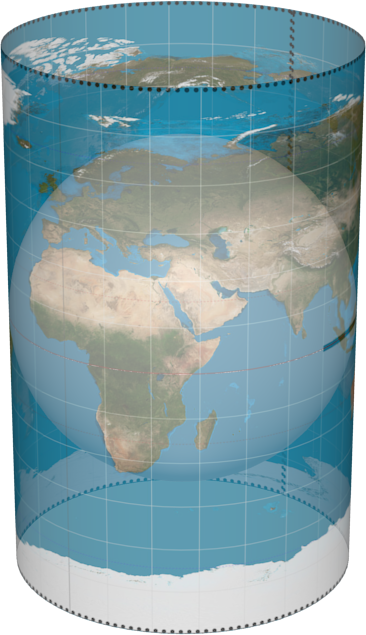
\includegraphics[width=\textwidth]{figures/map_projection/projection_geo.png}
    \end{subfigure}
    \caption{Geographic map projection.}
    \label{fig:proj_equi}
\end{figure}

\paragraph{Geocentric projection}
The simplest geographic parameterization uses geocentric coordinates. Here the latitude and longitude are defined as the angle between a vector from the origin to a point on the ellipsoid surface, and the $xy-$ and $xz-$planes respectively.

\paragraph{Geodetic projection}
The equirectangular cylindrical projection, using geodetic coordinates, is another variety of the geographic coordinate systems where the distance differential along the latitude $\partial \phi$ maps linearly to the latitude differential of the projected coordinates of the map.

Figure \ref{fig:geodetic} shows the difference between geocentric latitudes, $\phi_c$ and geodetic latitudes, $\phi_d$ for a point $\vec{p}$ on the surface of an ellipsoid. The figure also shows the difference between geocentric and geodetic surface normals, $\hat{n_c}$ and $\hat{n_d}$, respectively. 

\begin{figure}[htbp]
\centering
\begin{picture}(130,130)
    \put(0,0){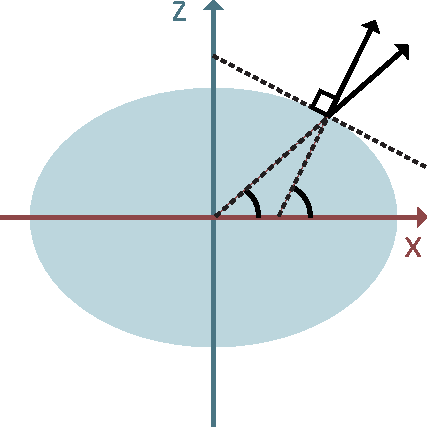
\includegraphics[width=0.35\textwidth]{figures/geodetic_geocentric.pdf}}
    \put(112,97){$\vec{p}$}
    \put(130,107){$\hat{n}_c$}
    \put(100, 130){$\hat{n}_d$}
    \put(100, 75){$\phi_d$}
    \put(82, 75){$\phi_c$}
    \label{fig:proj_equirectangular}
\end{picture}
\caption{Difference between geocentric and geodetic latitudes.}
\label{fig:geodetic}
\end{figure}

In the case of perfect spheres, geocentric and geodetic projections of any point will yield the same result.

Geodetic coordinates are among the most commonly used geo referenced coordinate systems when mapping ellipsoids to two dimensions. Latitudinal distances are preserved after the coordinate transform. This is important for a map projection standard that can be used for both spheres and for ellipsoids to avoid distortions that will appear if the map is defined for a specific ellipsoid and then projected on a slightly different one.

Equirectangular projections does not require specific ellipsoids to avoid distorsions on the mapped globe. The result of the wide usage is that many map providers choose to provide 2D maps defined in this coordinate system.

Cozzi and Ring describes the transform from geodetic coordinates in the ellipsoid class \cite[p. 25]{cozzi11}. For the Earth, the most commonly used geodetic coordinate space is defined in the EPSG:4326 standard where the WGS84 ellipsoid is used.

\subsubsection{Mercator Projection}

The mercator projection is a cylindrical projection widely used for presenting global maps in unwrapped form. The mercator projection preserves the horizontal to vertical ratio for small objects on the map. Hence, the mercator is a conformal projection in contrast to the geocentric and geodetic projections, which results in a non unit value in the ratio between the longitudinal and latitudinal differentials, see figure \ref{fig:mercator}.

\begin{figure}[htbp]
    \centering
    \begin{subfigure}[bt]{0.3\textwidth}
        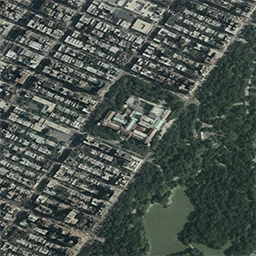
\includegraphics[width=\textwidth]{figures/central_park_equirectangular.png}
	\caption{The equirectangular projection is not conformal.}
    \end{subfigure}
    \qquad
    \begin{subfigure}[bt]{0.3\textwidth}
        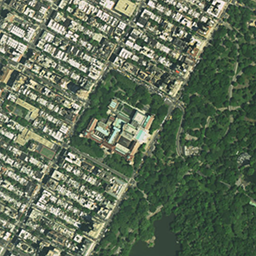
\includegraphics[width=\textwidth]{figures/central_park_mercator.png}
        \caption{The mercator projection is conformal and preserves aspect ratio.}
    \end{subfigure}
    \caption{Unwrapped equirectangular and mercator projections.}
    \label{fig:mercator}
\end{figure}

The mercator projection compensates for the longitudinal distortion by introducing a latitudinal distortion as well. Due to the polar singularities which lead to infinite latitudes at the poles when $\phi_d = \pm 90$, the domain of definition for the latitudes need to be constrained in mercator projection, see figure mercator.

\begin{figure}[htbp]
    \centering
    \begin{subfigure}[bt]{0.4\textwidth}
        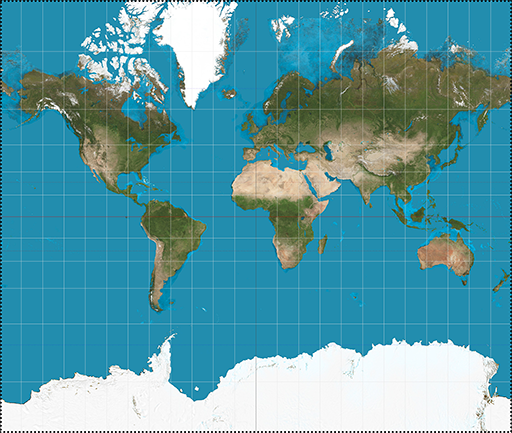
\includegraphics[width=\textwidth]{figures/developable_projected/mercator.png}
    \end{subfigure}
    \qquad
    \begin{subfigure}[bt]{0.15\textwidth}
        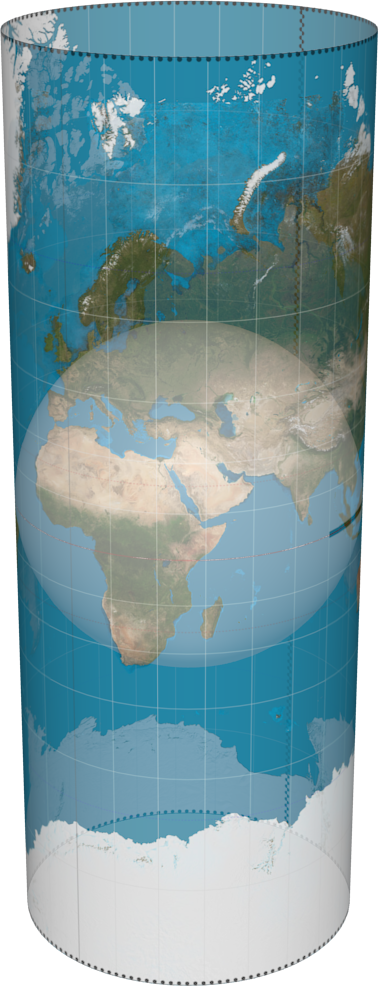
\includegraphics[width=\textwidth]{figures/map_projection/projection_mercator.png}
    \end{subfigure}
    \caption{Mercator projection.}
    \label{fig:proj_mercator}
\end{figure}

The EPSG:3857 standard for mercator projection of the Earth, also known as web mercator, constrains the domain to $\phi \in [-85.06, 85.06]$. The standard uses a different projection that does not diverge at the polar regions. Web mercator is used by most online web map applications including Google Maps, Bing Maps, OpenStreetMap, Mapquest, Esri and Mapbox \cite{battersby14}.

\subsubsection{Cube Map}

Cube maps lack the polar singularities apparent in geographic parameterizations. The parameterized coordinates are often discretized to the six sides of the cube, but they can also map directly to a global representation of an unwrapped cube, see figure \ref{fig:proj_cube}.

\begin{figure}[htbp]
    \centering
    \begin{subfigure}[bt]{0.4\textwidth}
        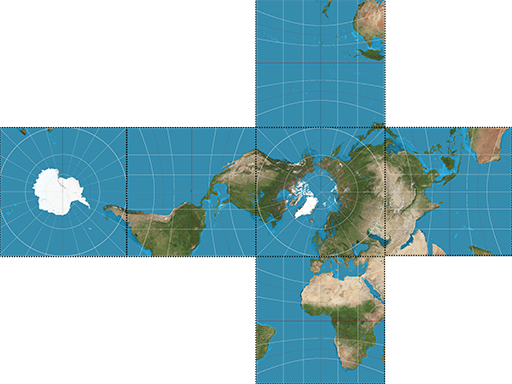
\includegraphics[width=\textwidth]{figures/developable_projected/cube_map.png}
    \end{subfigure}
    \qquad
    \begin{subfigure}[bt]{0.15\textwidth}
        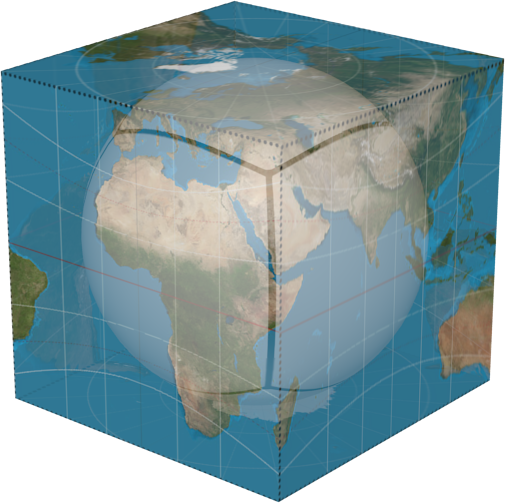
\includegraphics[width=\textwidth]{figures/map_projection/projection_cube.png}
    \end{subfigure}
    \caption{Cube map projection.}
    \label{fig:proj_cube}
\end{figure}

Due to the traditions of map projections this is not a common format used for map services so reprojection from a more common format is often required.

There are different cube map projections with different amount of area- and aspect distortions. Dimitrijevi\'{c} and Ran\v{c}i\'{c} mention and compares spherical cube, adjusted spherical cube, Outerra spherical cube and quadrilateralized spherical cube \cite{dimi15}.

\subsubsection{Tessellated Octahedral Adaptive Subdivision Transform}

The Tessellated Octahedral Adaptive Subdivision Transform (TOAST) map format used in the globe browsing of Microsoft's World Wide Telescope works together with the HTM tessellation \cite{toast}. Each triangular segment of the TOAST map maps linearly to a triangle of a sphere that is tessellated as an octahedron and subdivided to form a sphere, see figure \ref{fig:proj_toast}.

\begin{figure}[htbp]
    \centering
    \begin{subfigure}[bt]{0.3\textwidth}
        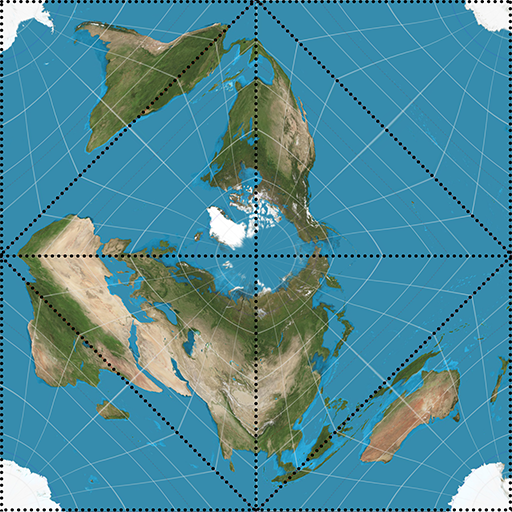
\includegraphics[width=\textwidth]{figures/developable_projected/toast.png}
    \end{subfigure}
    \qquad
    \begin{subfigure}[bt]{0.2\textwidth}
        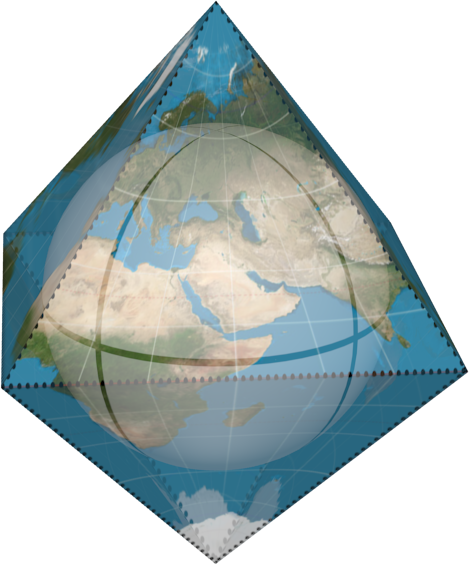
\includegraphics[width=\textwidth]{figures/map_projection/projection_toast.png}
    \end{subfigure}
    \caption{TOAST map projection.}
    \label{fig:proj_toast}
\end{figure}

The TOAST format is just as the cube maps not a very well supported format for map providers and harder to use together with some of the most common level of detail approaches due to the fact that most of them are optimized for rectangular and not triangular map tiles.

\subsubsection{Hierarchical Equal Area IsoLatitude Pixelation}

The map projection that is used for the HEALPix tessellation is equal-area as the name suggests. Figure \ref{fig:proj_healpix} shows how the map wraps onto the sphere. The positive aspect about HEALPix compared to the TOAST format is that the map is tiled into quads and not triangles which means that it is better suitable for the chunked lod \cite{cozzi11} algorithm. The map format is used by the Sloan Digital Sky Survey for mapping the cosmic microwave background radiation but is otherwise an uncommon format when it comes to map services. That means that the maps need to be reprojected from the more common formats for wider support.

\begin{figure}[htbp]
    \centering
    \begin{subfigure}[bt]{0.5\textwidth}
        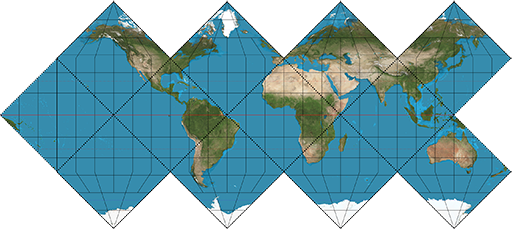
\includegraphics[width=\textwidth]{figures/developable_projected/healpix.png}
    \end{subfigure}
    \qquad
    \begin{subfigure}[bt]{0.2\textwidth}
        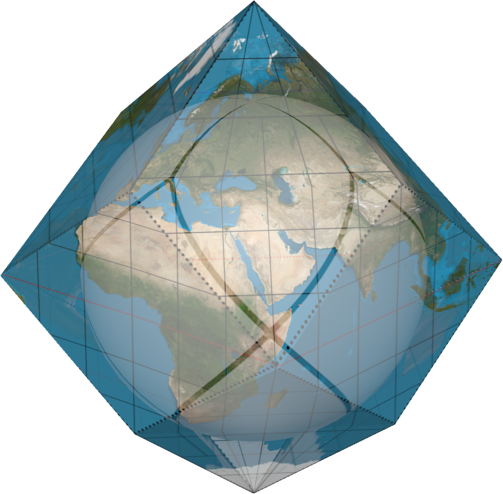
\includegraphics[width=\textwidth]{figures/map_projection/projection_healpix.png}
    \end{subfigure}
    \caption{HEALPix map projection.}
    \label{fig:proj_healpix}
\end{figure}

\subsubsection{Polar Projections}

For parameterization of limited parts of the globe, such as the isolated poles, there are different projections to consider. Most common are different types of azimuthal projections. These projections are defined by projecting all points of the map through a common intersection point and onto a flat surface. The Gnomonic projection maps all great circle segments (geodesics) to straight lines by having the common intersection point in the center of the globe.

Stereographic projections are defined when the common intersection point is positioned on the surface of the globe on the opposite side of the pole to project. Polar stereographic projections are used to parameterize the surface of the poles of the Earth. The standards EPSG:3413 and EPSG:3031 define the stereographic projections for the North Pole and the South Pole respectively.

Dimitrijevi\'{c} and Ran\v{c}i\'{c} uses another polar coordinate system to reproject from geodetic coordinates in runtime. The transformation is a rotation of 90 degrees around the global $x-$axis so that the resulting parametric coordinates of the pole are given in their own geographic space with the main meridian as equator. This projection is also known as a Cassini projection and it can be both defined for spheres as well as generalized to ellipsoids. Polar projections are shown in figure \ref{fig:proj_polar}.

\begin{figure}[htbp]
    \centering
    \begin{subfigure}[b]{0.3\textwidth}
        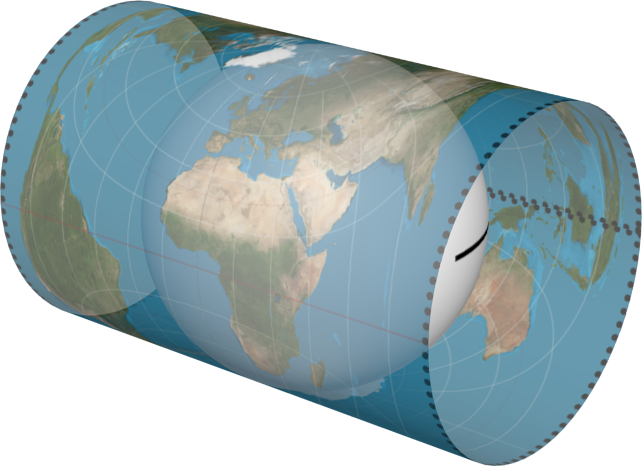
\includegraphics[width=\textwidth]{figures/map_projection/projection_cassini.png}
    	\caption{Cassini}
    \end{subfigure}
    ~
    \begin{subfigure}[b]{0.3\textwidth}
        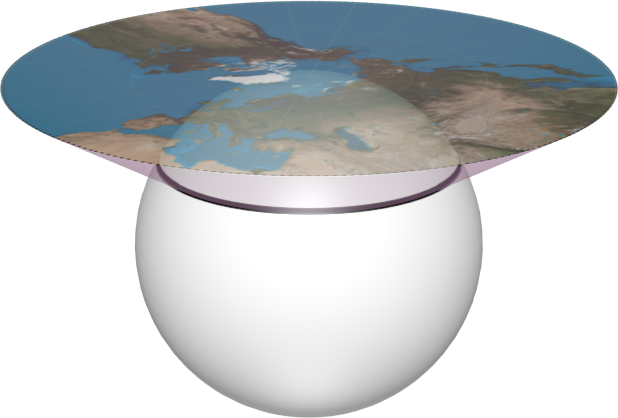
\includegraphics[width=\textwidth]{figures/map_projection/projection_gnomonic.png}
        \caption{Gnomonic}
    \end{subfigure}
    ~
    \begin{subfigure}[b]{0.3\textwidth}
        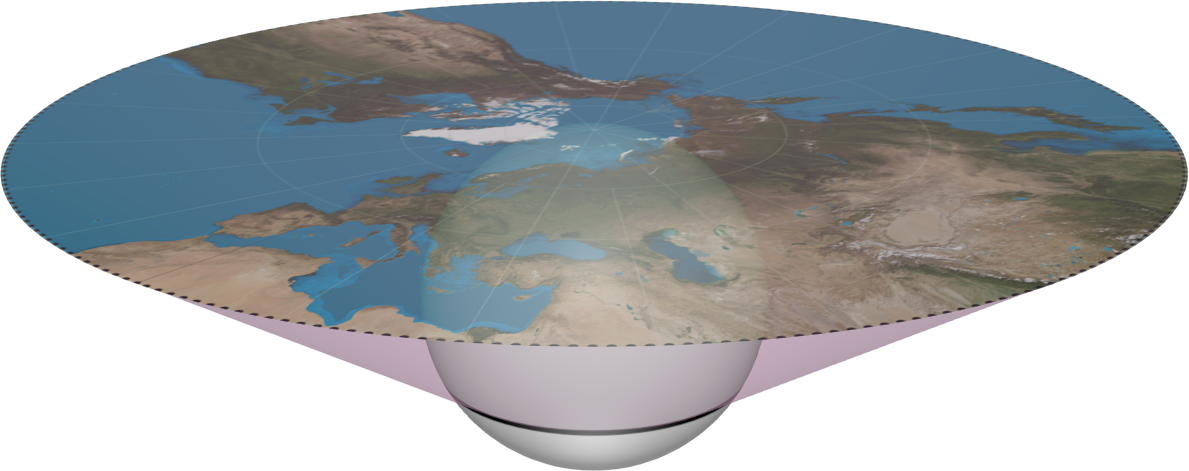
\includegraphics[width=\textwidth]{figures/map_projection/projection_stereographic.png}
    	\caption{Stereographic}
    \end{subfigure}
    \caption{Polar map projections.}
    \label{fig:proj_polar}
\end{figure}

\section{Dynamic Level of Detail}
Dynamic level of detail (LOD) is an important part in handling the extensive amount of data used in an out of core rendering software. The goal is to maximize the visual information on screen while minimizing the workload. In their book Rendering virtual 3D globes, Cozzi and Ring describes LOD rendering algorithms by three typical steps. \cite[p. 367]{cozzi11}

\begin{enumerate}
    \item Generation - Create versions at different level of detail of a model
    \item Selection - Choose a version based on some criteria or error metric (e.g., distance to object or the projected area it occupies on the screen)
    \item Switching - Transitions from one version to another in order to avoid noticing of the change in LOD known as popping artifacts.
\end{enumerate}

There are different types of LOD approaches for terrain rendering, and a suitable approach should be chosen based on characteristics of the terrain. Terrains can for example be restricted to being represented as height maps - a characteristic that can be exploited by the rendering algorithm. Cozzi and Ring describe the following three categories of LOD approaches: Discrete Level of Detail, Continuous Level of Detail and Hierarchical Level of Detail \cite[p. 368-371]{cozzi11}.

\subsection{Discrete Level of Detail}
In the Discrete Level Of Detail (DLOD) approach, multiple different representations of the terrain are created at different resolutions. DLOD is arguably the most simple LOD algorithm. It works not only for digital terrain models, but for arbitrary meshes. The set of terrain representations can either be predefined or generated using mesh simplification algorithms.

\begin{figure}[htbp]
    \centering
    \begin{subfigure}[bt]{0.9\textwidth}
        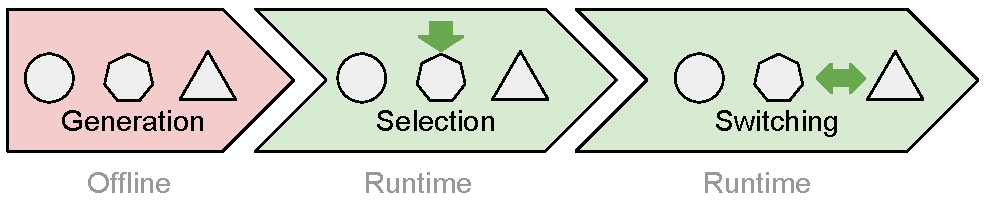
\includegraphics[width=\textwidth]{figures/lod/lod_overview.pdf}
    \end{subfigure}
    \caption{DLOD. Generate offline, select and switch at runtime.}
    \label{fig:lod}
\end{figure}

\begin{figure}
    \centering
    \begin{subfigure}[b]{0.2\textwidth}
        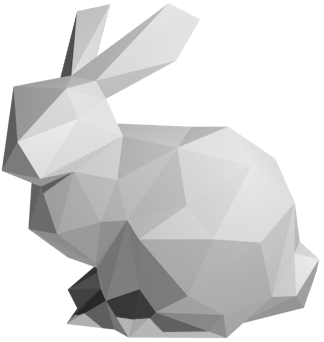
\includegraphics[width=\textwidth]{figures/lod/decimation3.png}
    \end{subfigure}
    ~ %add desired spacing between images, e. g. ~, \quad, \qquad, \hfill etc. 
      %(or a blank line to force the subfigure onto a new line)
    \begin{subfigure}[b]{0.2\textwidth}
        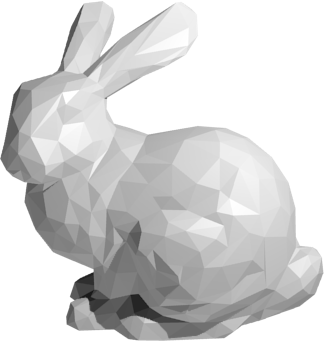
\includegraphics[width=\textwidth]{figures/lod/decimation2.png}
    \end{subfigure}
    ~ %add desired spacing between images, e. g. ~, \quad, \qquad, \hfill etc. 
    %(or a blank line to force the subfigure onto a new line)
    \begin{subfigure}[b]{0.2\textwidth}
        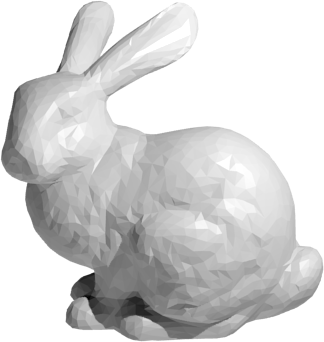
\includegraphics[width=\textwidth]{figures/lod/decimation1.png}
    \end{subfigure}
    \caption{A range of predefined meshes with increasing resolution}
    \label{fig:dlod}
\end{figure}

At run time, the main objective is to select one (or generate) a suitable representation. This approach does not provide any means of dealing with large scale datasets, which makes it unsuitable for globe rendering (ref virtual globes).


\subsection{Continuous Level of Detail}
The continuous LOD (CLOD) approach represents a model in a way that allows the resolution to be selected arbitrary. This is usually implemented by a base mesh combined with a sequence of operations that successively changes the level of detail of the model. Two typical such operations are ``edge collapse'' (removes two triangles from the mesh) and its inverse, ``vertex split'' (adds two triangles to the mesh) are illustrated in Figure \ref{fig:clod}.

\begin{figure}
    \centering
    \begin{subfigure}[b]{0.2\textwidth}
        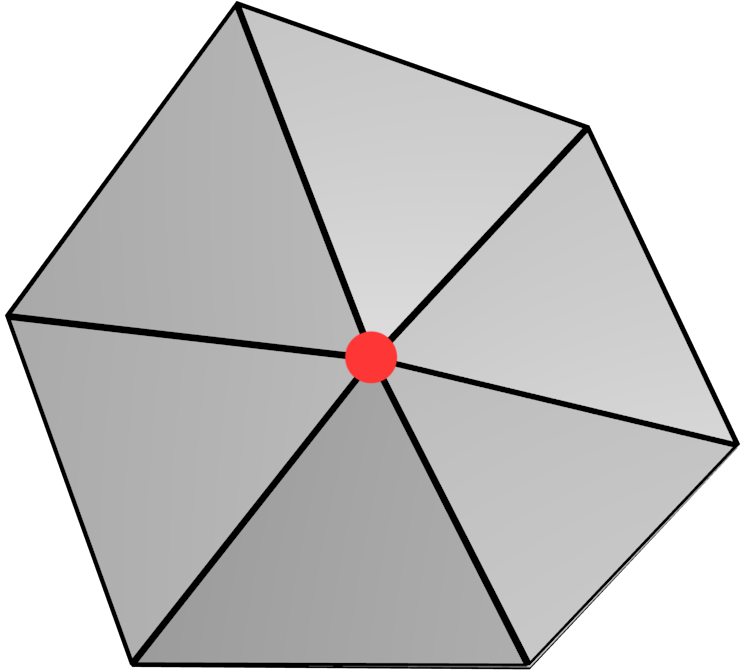
\includegraphics[width=\textwidth]{figures/lod/vertex_split1.png}
    \end{subfigure}
    ~ %add desired spacing between images, e. g. ~, \quad, \qquad, \hfill etc. 
      %(or a blank line to force the subfigure onto a new line)
    \begin{subfigure}[b]{0.2\textwidth}
        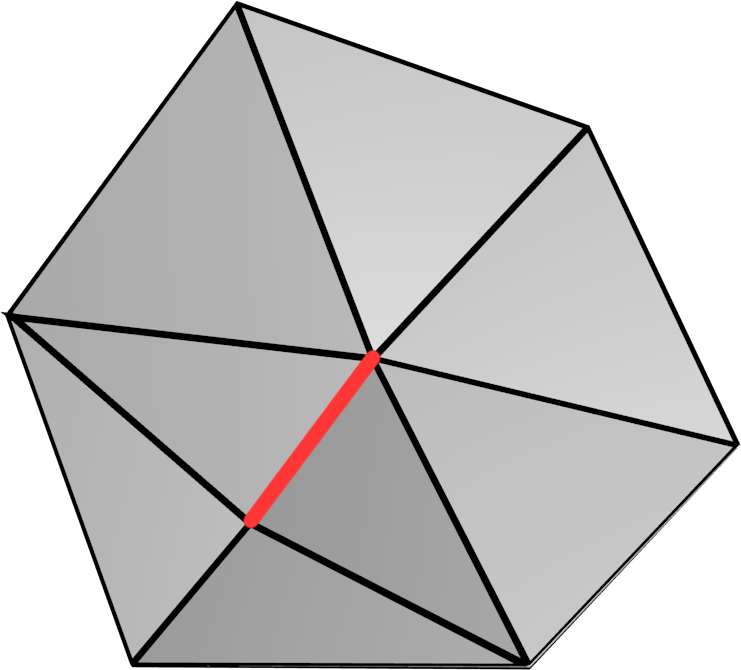
\includegraphics[width=\textwidth]{figures/lod/vertex_split2.png}
    \end{subfigure}
    \caption{Edge collapse in continous LOD}
    \label{fig:clod}
\end{figure}

According to Cozzi and Ring \cite[p. 368]{cozzi11} CLOD has previously been the most popular approach for rendering terrain at interactive rates, with implementations such as Real-time Optimally Adaptive Mesh (ROAM). The main reason CLOD algorithms are not widely employed these days is due to the increase in triangle throughput on modern GPUs, causing the CLOD operations done on the CPU in many cases to act as a bottleneck for the rendering time.

A special branch of CLOD worth mentioning is the so called infinite LOD. In this approach the terrain is represented by a mathematical function - an implicit surface. These functions can be defined by fractal algorithms and produce complex characteristics, or they can define simple geometric shapes such as spheres or ellipsoids. As every point on these types of surfaces are precisely defined, triangle meshes can be generated with no limit on the level of detail. This approach is not suitable for incorporating real world data, but it is used by terrain engines such as Outerra and Terragen to procedurally generate terrain at any desired level of detail \cite{outerraprocedural09}. 

\subsection{Hierarchical Level of Detail}
Hierarchical Level of Detail (HLOD) can be seen as a generalization of DLOD. HLOD algorithms operates on hierarchically arranged, predefined chunks of the full model. Each chunk is processed, stored and rendered separately. By doing this, HLOD approaches tackles the weaknesses of CLOD, essentially by doing the following.

\begin{enumerate}
    \item Reduce processing time on CPU: The only CPU task that HLOD algorithms has to deal with during runtime is to select a suitable subset of the predefined chunks for rendering. This is a relatively fast procedure in contrast to iteratively applying changes to the raw geometry, as done in CLOD.
    \item Reduce the data traffic to GPU: Data is uploaded to the GPU in larger batches but not very often, since the data is static and GPU caching can be done. With CLOD, the geometry data is updated on a per-frame basis, and can't be cached on the GPU. Being able to perform GPU caching allow HLOD to better minimize the traffic to the GPU.
\end{enumerate}

HLOD uses spatial hierarchical data structures such as quadtrees or octrees for storing the chunk data. The root node of the tree holds a full representation of the model at its lowest level of detail a one single chunk. At successive levels, the model is represented at a higher level of detail but divided up into several chunks. This concept is illustrated in Figure \ref{fig:hlod}.

\begin{figure}[htbp]
    \centering
    \begin{subfigure}[bt]{0.4\textwidth}
        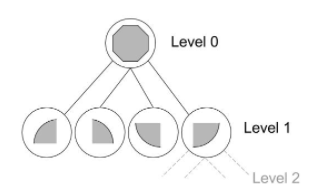
\includegraphics[width=\textwidth]{figures/lod/hlod_tmp.png}
    \end{subfigure}
    \caption{HLOD using a quadtree.}
    \label{fig:hlod}
\end{figure}

Generally, selecting all the chunks at a specific level in the tree yields a complete representation of the model. Furthermore, chunks may be selected from different levels for different parts of the model and still yield a full representation of the model. This allows for view dependent rendering of the model. Algorithm chunk selection describes pseudo code for recursively rendering the full model at view dependent level of detail.

\begin{algorithm}[htp]
  \SetKwFunction{RenderLOD}{}
  \SetKwProg{myalg}{RenderLOD}{}{}
  \myalg{\RenderLOD{Camera C, ChunkNode N}}{
  \eIf{ErrorMetric($C$, $N$) < threshold}{
        Render($N$, $C$)
    }{
        \For{$child$ \textbf{in} $children(N)$}{
            RenderLOD($child$, $C$)
        }
    }
  }{}
  \caption{Algorithm with procedure}
\end{algorithm} 

This example uses a depth first approach for rendering of chunks. Other common schemes for traversing the hierarchy are breadth first and inverse breadth first.

The algorithm traverses the tree and calculates an error metric at each node with respect to the current camera position. If the calculated error is larger than a certain threshold, the algorithm recursively repeats the procedure for all the chunk's children, which has higher level of detail. This general scheme can be used for rendering one-dimensional curves (using a binary tree structure), two-dimensional surfaces (using a quadtree) or volumes (using an octree).

Another key feature of HLOD as opposed to DLOD and CLOD is that it can naturally be integrated with out-of-core rendering, as chunks can be loaded into memory on-demand and thrown away when not needed.

%%%%%%%%%%%%%%%%%%%%%%%%%%%%%%%%%%%%%%%%%%%%%%%%%%%%%%%%%%%%%%%%%%%%%


\section{Level of Detail Algorithms for Globes}
A number of different LOD algorithms has been introduced for the purpose of globe rendering. Two common algorithms used are Chunked LOD and Geometry Clipmaps, as pointed out by Cozzi and Ring\cite{cozzi11}.

\subsection{Chunked LOD}
The Chunked LOD method fits into the category of a HLOD system and works by breaking down the surface of the globe into a quadtree of chunks. There are several different tiling schemes that can be used for spatially organizing the chunks. Some tiling schemes are defined as the ellipsoidal tessellation methods described under ``Tessellating the Ellipsoid''. 

\begin{figure}[htbp]
    \centering
    \begin{subfigure}[bt]{0.4\textwidth}
        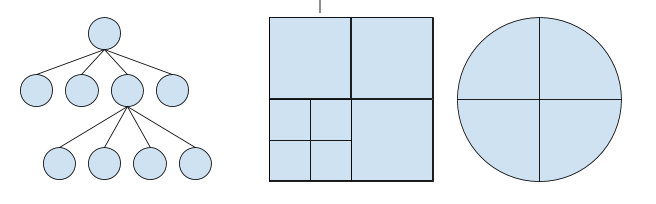
\includegraphics[width=\textwidth]{figures/chunkedlod/chunkedlodglobe.png}
    \end{subfigure}
    \caption{Chunk LOD for a globe}
    \label{fig:chunkedlod}
\end{figure}

Figure \ref{fig:chunkedlod} demonstrates the layout of chunks as they are mapped in geographic coordinates onto an ellipsoid representation of a globe.

\subsubsection{Chunks}
Chunks should store the following data:

\begin{enumerate}
    \item A mesh defining the terrain geometry (positions, normals, uv-coordinates). 
    \item A monotonic geometric error, based on the vertices distances to the fully detailed mesh. The children of a chunk should always have a smaller geometric error as they can better fit the highest level of detail model.
    \item A known bounding volume encapsulating the mesh and optimally all the chunk's children. This is used along with the geometric error metric when selecting suitable chunks for rendering.
\end{enumerate}

Depending on the implementation of the chunked LOD algorithm, these properties can be either calculated on the fly or preprocessed as suggested by Cozzi and Ring\cite[p. 447]{cozzi11}. Furthermore, the chunk mesh must fulfill two important requirements: 

\begin{enumerate}
    \item Have vertices defined in each corner of the mesh
    \item Have defined edges along its sides such that when two adjacent chunks are rendered next to each other, there is no gap in between them. See subsection Cracks below for more about this topic
\end{enumerate}

Cozzi and Ring suggests rectangular chunk meshes, although triangular tiling schemes (such as HTM) can also be used \cite{htm}.

\subsubsection{Selection}
There are different ways of selecting chunks for rendering, based on different ways of calculating an error metric for each chunk. (See Algorithm chunk selection in HLOD section). As an example, a very simple view-dependent error metric could use the chunk size divided by the distance between the camera and the chunk. If the ratio is larger than a certain threshold, the algorithm should instead consider each of the chunk's children by splitting the chunk into four. Another approach is to consider the actual visual effect on the screen. With a geometric error stored in each chunk, it is possible to calculate a maximum screen space error in pixels with respect to the current camera view. [Cozzi and Ring] This gives the user the convenience of being able to specify a maximum pixel error threshold.

\subsubsection{Culling}
An important thing to consider when dealing with chunks of a virtual globe is the fact that the chunks that are selected for rendering might not actually be visible on the screen. Needless to say, this is a waste of computational power and by eliminating these unnecessary draw calls, the performance of the globe renderer can be increased.

\paragraph{Camera frustum culling} This is done by testing a bounding box of the chunk for intersection with the camera frustum. If the chunk is completely outside the frustum, the chunk can safely be culled as it will not be visible in the rendered image. See Figure \ref{fig:frustumculling}.

\begin{figure}[htbp]
    \centering
    \begin{subfigure}[bt]{0.4\textwidth}
        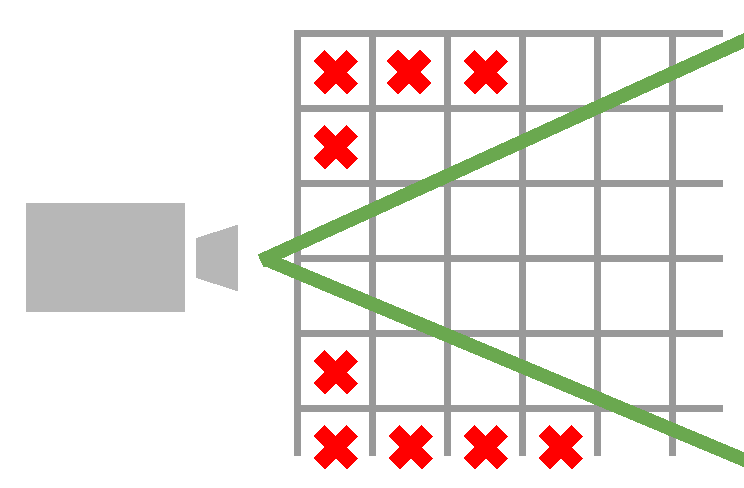
\includegraphics[width=\textwidth]{figures/chunkedlod/frustumculling.pdf}
    \end{subfigure}
    \caption{Frustum culling}
    \label{fig:frustumculling}
\end{figure}

\paragraph{Horizon culling} Even after camera frustum culling there are chunks that still do not contribute to the rendered image. Figure \ref{fig:horizonculling} illustrates that most of a globe is actually invisible to any observer. This can be used as a basis for culling some of the remaining chunks. 

\begin{figure}[htbp]
    \centering
    \begin{subfigure}[bt]{0.4\textwidth}
        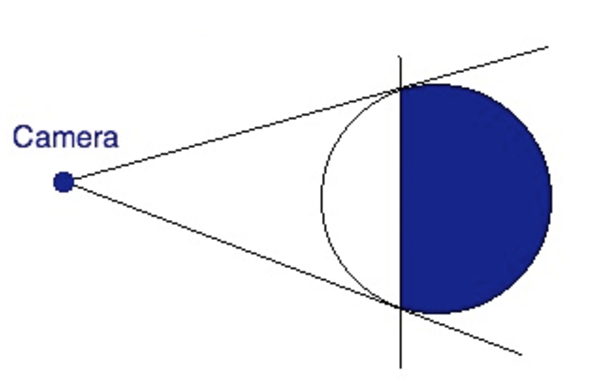
\includegraphics[width=\textwidth]{figures/chunkedlod/horizonculling.png}
    \end{subfigure}
    \caption{Horizon culling}
    \label{fig:horizonculling}
\end{figure}


\subsubsection{Switching}
Even with sophisticated methods for selecting and culling chunks, users of a globe rendering system will notice ``popping'' effects as chunks are splitted and merged. Even when chunks can be selected in a way that guarantees a maximum pixel error per vertex, the fact that full areas of multiple triangles are replaced all at once causes a drastic change in the rendered view. Even when the updates are small per vertex, the update of whole chunk areas may be easily noticed. This is what is referred to as popping.

Minimizing popping artifacts are typically done by smoothly transitioning between levels over time. Cozzi and Ring suggest an approach where along with each vertex, a delta offset is also stored\cite[p. 451]{cozzi11}. This delta offset stores the difference between the chunk itself and the same region within the parent chunk. Using this difference, new vertices can be placed on already defiend edges, and then interpolated into their actual positions. Figure switch below illustrates the idea.

\begin{figure}[htbp]
    \centering
    \begin{subfigure}[bt]{0.7\textwidth}
        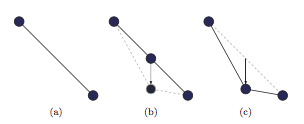
\includegraphics[width=\textwidth]{figures/chunkedlod/switching.png}
    \end{subfigure}
    \caption{a) An edge at chunk level i-1. b) The same edge after level i has been selected. c) The new vertex is interpolated into its true place.}
    \label{fig:lodswitch}
\end{figure}

The interpolation parameter can be based on the distance to the camera or time based animation.

\subsubsection{Cracks and skirts}
As chunks are tiled and rendered next to each other, it is desireable to make the borders between chunks as unnoticeable as possible. Even though the chunk meshes are generated according to the requirements mentioned in the Chunk subsection above, it is not possible to guarantee a watertight edge between two adjacent chunks of different LOD. Where adjacent chunks have different detail level, so called T-junctions till emerge. These T-junctions cause cracks between the chunks as an unwanted visual artifact.

The easiest way to tackle this issue is not to try to remove the cracks, but instead try to hide them. The most common approach hides the cracks by simply adding an extra layer of vertices to the sides of sides of the mesh. This extra layer of vertices, which are also known a skirt, is offset down vertically, as illustrated in figure \ref{fig:skirts}. 

By adding skirts to the chunk meshes, the model will not be rendered with visible holes in it. Instead, the holes will be filled up with textured triangles.

\begin{figure}[htbp]
    \centering
    \begin{subfigure}[bt]{0.4\textwidth}
        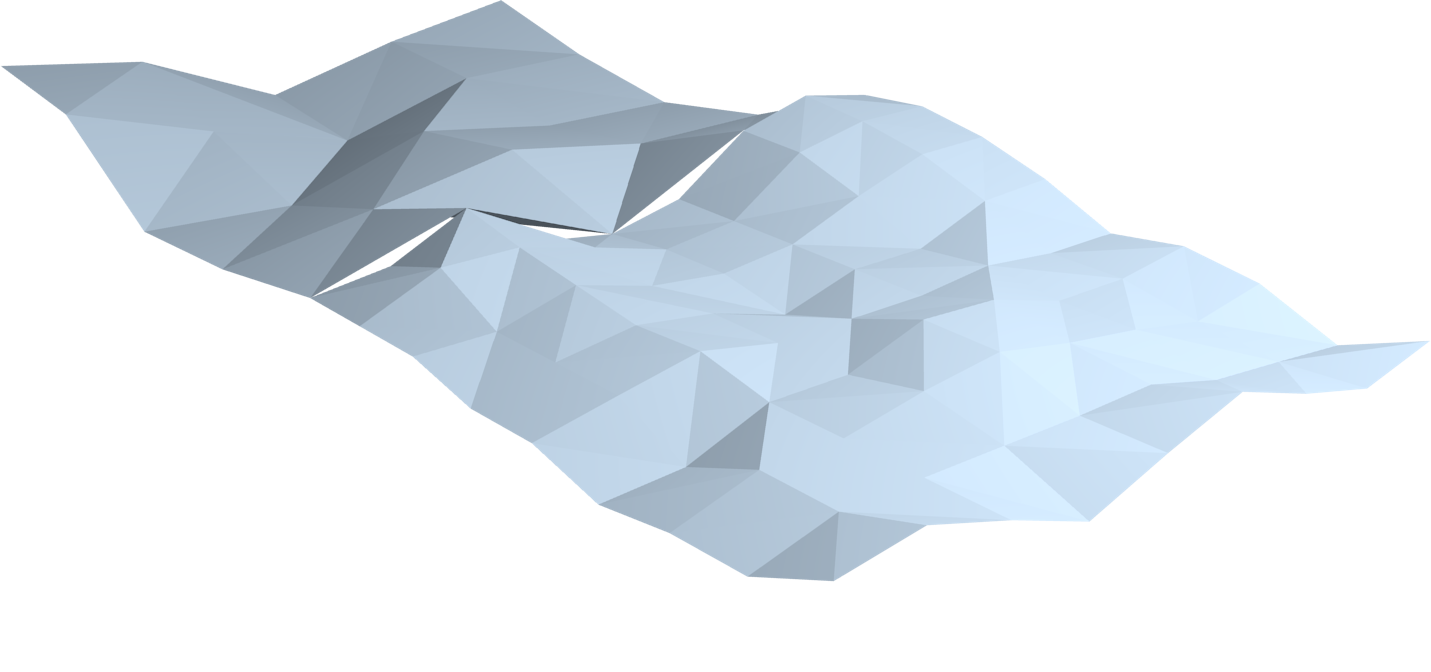
\includegraphics[width=\textwidth]{figures/chunkedlod/skirts_without.png}
        \caption{No skirts.}
    \end{subfigure}
    \begin{subfigure}[bt]{0.4\textwidth}
        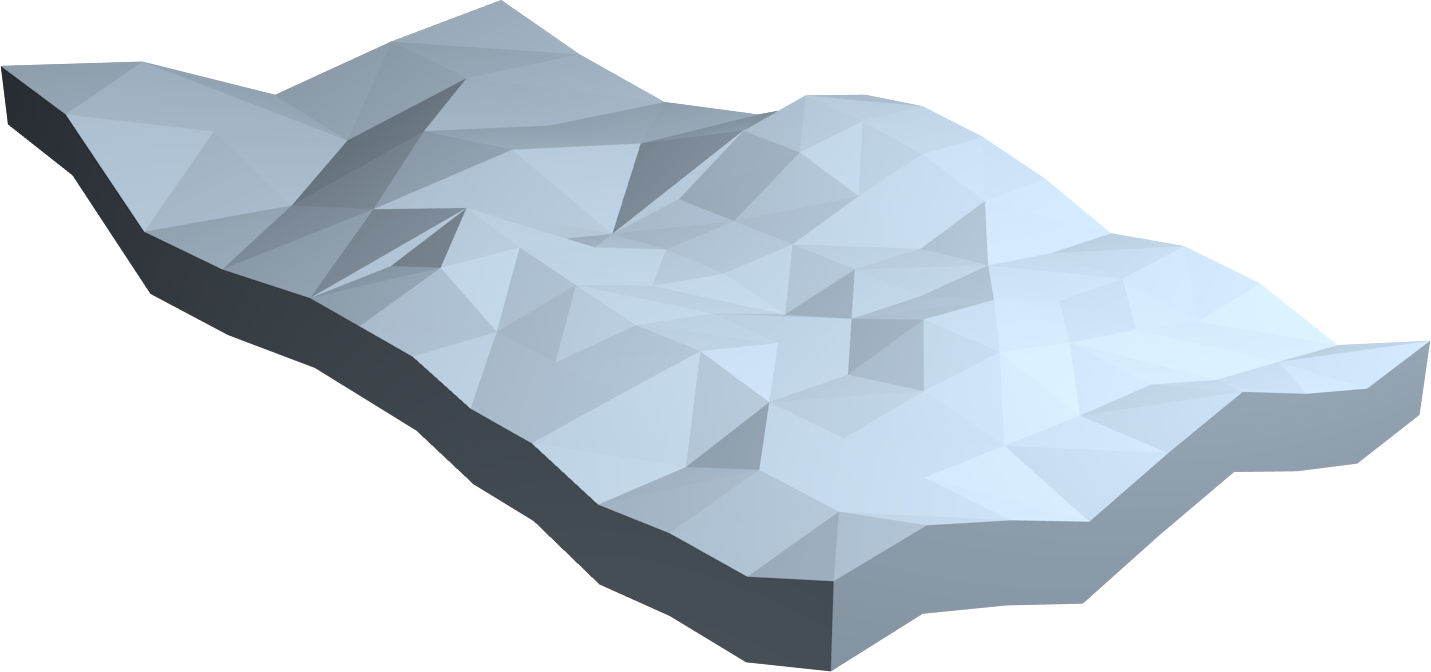
\includegraphics[width=\textwidth]{figures/chunkedlod/skirts_with.png}
        \caption{Skirts}
    \end{subfigure}
    \caption{Chunks with skirts hide the undesired cracks between them.}
    \label{fig:skirts}
\end{figure}


\subsection{Geometry Clipmaps}
A clipmap texture is a dynamic mip map where each image in the so called clipmap stack is clipped down to a constant size. This reduces the amount of memory of the whole texture to increase linearly instead of exponentially with the number of overlays for LOD textures. Figure \ref{fig:clipmapmipmap} a shows the difference between the amount of texture data stored in a regular mip map compared to a clip map.

\begin{figure}[htbp]
    \centering
    \begin{subfigure}[bt]{0.8\textwidth}
        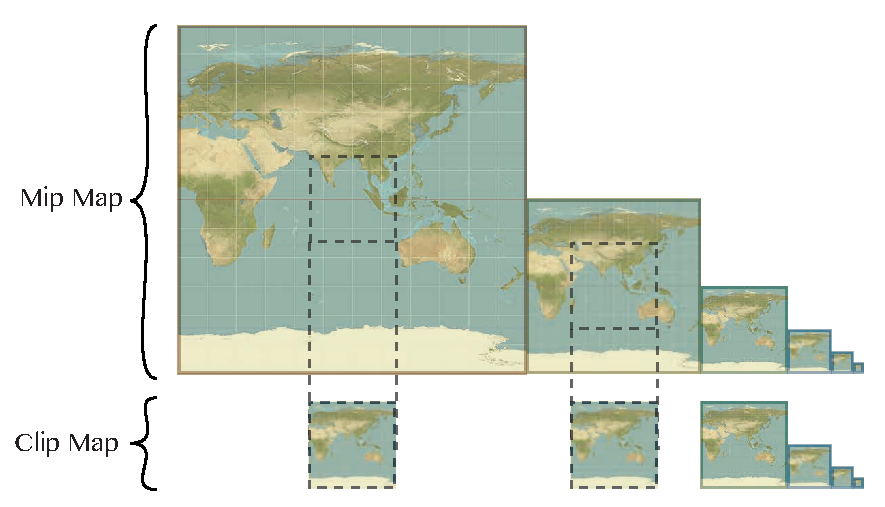
\includegraphics[width=\textwidth]{figures/geometryclipmap/clipmap_mipmap.pdf}
    \end{subfigure}
    \caption{Comparison of mip maps and clip maps}
    \label{fig:clipmapmipmap}
\end{figure}

The idea of clipmaps can be applied not only to textures but also to geometries. By representing a terrain by a stack of clipmap geometries of different size, the resolution increases closer to the virtual camera, as illustrated in Figure \ref{fig:clipmapgeometry}. As the view point moves around, the grids updates their vertex positions accordingly to keep the grind centered in the geometry clipmap stack. The position of each of the levels of the clip map geometries snaps to a discrete coordinate grid with cell sizes equal to the distance between two adjacent vertices.

\begin{figure}[htbp]
    \centering
    \begin{subfigure}[bt]{0.6\textwidth}
        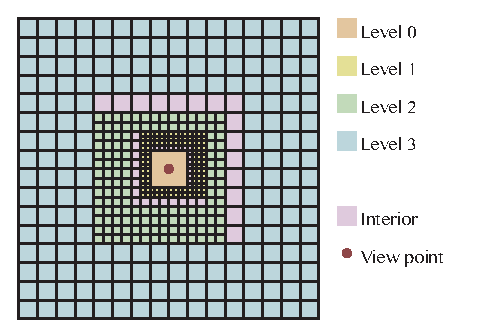
\includegraphics[width=\textwidth]{figures/geometryclipmap/clipmap_geo.pdf}
    \end{subfigure}
    \caption{The Geometry Clipmaps follow the view point.}
    \label{fig:clipmapgeometry}
\end{figure}

Geometry clipmaps limits the terrain representation to be in the form of height maps. This is because the clipmap geometry moves around when the focus point changes and since the underlying terrain should not follow the camera position, the clipmap geometries requires vertex shader texture fetching. The texture coordinates are offset as the geometry clipmap moves to follow the focus point.

One of the main selling points for geometry clipmaps is the decrease in CPU workload and the increase in GPU triangle throughput. There is no need to traverse a hierarchical structure such a quadtree. The number of draw calls will remain equal the number of clip maps instead of the number of chunks which is often larger. The framerate will also be relatively consistent if the number of layers in the clipmap stack remains constant.

\subsubsection{2D Grid Geometry Clipmaps}
Using geometry clipmaps to achieve dynamic level of detail for a height mapped grid was proposed by Dimitrijevi\'{c} and Ran\v{c}i\'{c} \cite{dimi15}. The method is limited to rendering of equirectangular grids. When considering the ellipsoidal shape of a globe, the clipmap grid can be represented in geographic coordinates mapped on an ellipsoid where the map texture coordinates in the longitudinal direction wraps around the anti meridian. Rendering the clipmap close to the poles however will lead to polar pinching which breaks the globe as illustrated in Figure \ref{fig:mipclip}.

\begin{figure}[htbp]
    \centering
    \begin{subfigure}[bt]{0.25\textwidth}
        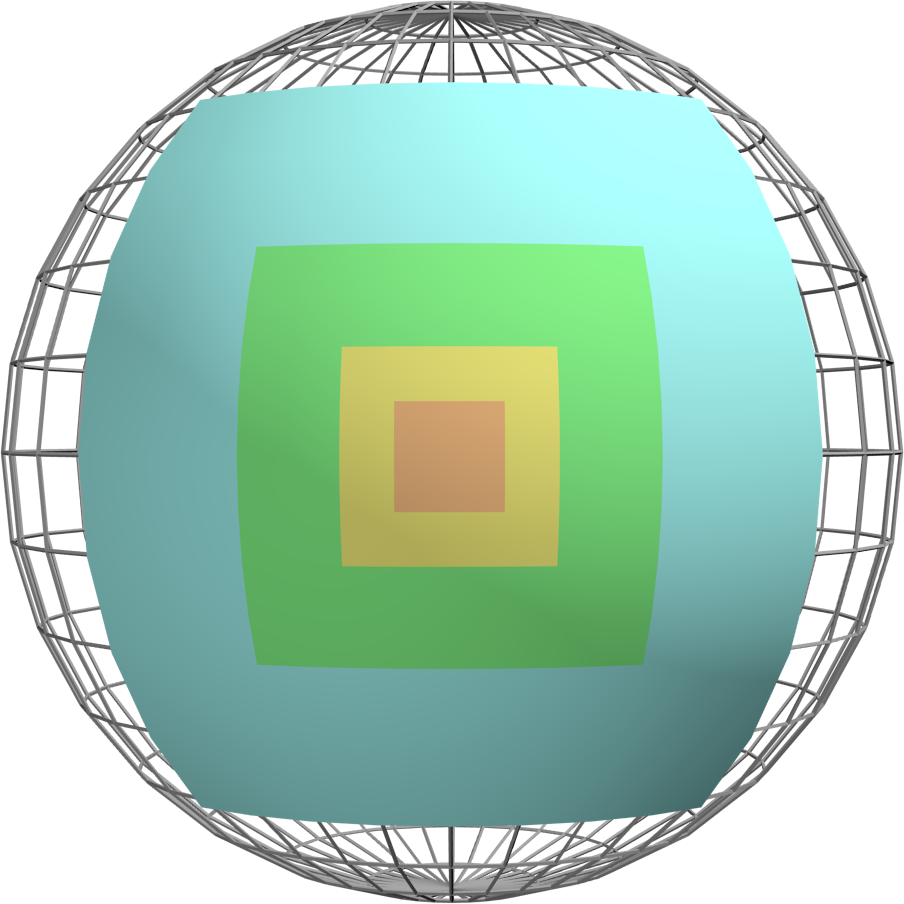
\includegraphics[width=\textwidth]{figures/geometryclipmap/clipmap1.png}
        \caption{Near the equator}
    \end{subfigure}
    \quad
    \begin{subfigure}[bt]{0.25\textwidth}
        \includegraphics[width=\textwidth]{figures/geometryclipmap/clipmap2.png}
        \caption{Near a pole}
    \end{subfigure}
    \caption{Geometry Clipmaps on a geographic grid cause pinching effect around the poles, which needs to be handled explicitly.}
    \label{fig:mipclip}
\end{figure}

Clipmap grids can also be used to model a spherical cube representation of a globe to avoid polar issues. This requires six clipmap partitions; one for each side of the cube.

\subsubsection{Spherical Clipmaps}
Spherical clipmaps takes advantage of the fact that no observer will ever see more than half a globe at any time. The vertices of the clipmap are described in polar coordinates with the center of the grid always following the camera position. The coordinates of the vertices will therefore not have any correspondence to texture coordinates which is why the algorithm is not widely adopted\cite{dimi15}. 

\subsubsection{Ellipsoidal Clipmaps}
Dimitrijevi\'{c} and Ran\v{c}i\'{c} introduces ellipsoidal clipmaps as a level of detail rendering method for globes \cite{dimi15}. It uses a geographic grid for the polar regions of the globe and solves the polar issues with the use of polar caps. The advantages compared to spherical cube clipmaps is that it uses the well known geographic map projection and reduces the number of geometry clipmap partitions from six to two. The globe is divided into one equatorial region and two polar regions. If the distance is close enough to the globe (3,000 km above the surface for the Earth), a maximum of two partitions is needed at any time \cite{dimi15}.

The area distortion and the aspect distortion of the map projection of the ellipsoidal clipmap method is low compared to cube map projections but requires extra care to hide the discontinuities that appear at the edges between the equatorial and polar partitions \cite{dimi15}.

The most generally used level of detail algorithms of today are chunked LOD and varieties of geometry clipmaps. Cozzi and Ring compare the algorithms and gives the advantages and disadvantages depending on the needs of the globe browsing software. The main differences are summarized and presented in Table \ref{table:lodcomparison} \cite[p. 464]{cozzi11}. 
\begin{center}
  \begin{table}
  \caption[]{Comparing geometry clipmapping and chunked LOD}
    \label{table:lodcomparison}
  \begin{tabular}{| r | c | c |}
    \hline
                            & \textbf{Geometry Clipmaps} & \textbf{Chunked LOD} \\ \hline

    Preprocessing           & Minimal           & Extensive \\
    Mesh Flexibility        & None              & Good \\
    Triangle Count          & High              & Lower \\
    Ellipsoid Mapping       & Challenging       & Straightforward \\
    Error Control           & Poor              & Excellent \\
    Frame-Rate Consistency  & Excellent         & Poor \\
    Mesh Continuity         & Excellent         & Poor \\
    Terrain Data Size       & Small             & Large \\
    Legacy Hardware Support & Poor              & Good \\
    \hline
  \end{tabular}
  \end{table}
\end{center}

%%%%%%%%%%%%%%%%%%%%%%%%%%%%%%%%%%%%%%%%%%%%%%%%%%%%%%%%%%%%%%%%%%%


\section{Large Scale Map Datasets}

Global maps with high level of detail can easily become too large to be stored and read locally on a single machine. A common way of storing large maps is by representing them using several overviews. An overview is a map representing the same geographical area as the original map but containing only one fourth as many pixels just like a lower level of a mip map texture. Figure \ref{fig:overview} shows how the size of the maps in raster coordinates decreases with the overview number.

\begin{figure}[htbp]
    \centering
    \begin{picture}(130,60)
        \put(0,0){\includegraphics[width=0.5\textwidth]{figures/overview.pdf}}
        \put(-50,50){Overview:}
        \put(45,50){0}
        \put(127,50){1}
        \put(176,50){n}
        \put(-5,25){$y$}
        \put(45,-5){$x$}
    \put(100,35){$\frac{y}{2}$}
    \put(127,15){$\frac{x}{2}$}
    \put(155,37){$\frac{y}{2^n}$}
        \put(176,25){$\frac{x}{2^n}$}

        \label{fig:proj_equirectangular}
    \end{picture}
    \caption{The size of the map is decreasing exponentially with the overview.}
    \label{fig:overview}
\end{figure}

The physical disk space of large global map datasets is often measured in terabytes or even petabytes. In order to deal with such large datasets, web based services allow users to specify only parts of the map to download at a time. This is an important aspect in the out of core rendering required for globe visualization.

\subsection{Web Map Services}

To standardize web requests for map data, the Open GIS Consortium (OGS) specified a web map service interface \cite{wms06} and from that, specifications of several other map service interfaces have followed. The most common standards are Web Map Service (WMS), Tile Map Service (TMS) and Web Map Tile Service (WMTS). Some more specific examples of WMS-like services are WorldWind, VirtualEarth and AGS. The last three are not covered in this thesis.

\subsubsection{WMS}

The WMS interface produces maps as image files with well defined geographic and dimensional parameters. The image files can have different format and compression depending on the provider. A WMS server has the ability to dynamically produce map patches of arbitrary size which puts some load on the server side \cite{wms06}. The basic elements supported by all WMS providers are the \emph{GetCapabilities} and the \emph{GetMap} operations. \emph{GetCapabilities} gives information about the available maps on the server and their corresponding geo referenced metadata. The \emph{GetMap} operation returns the map or a part of the map as an image file.

The structure of a WMS request using HTTP GET is of the form \\ \texttt{http://host\lbrack:port\rbrack/path\lbrack?\{name\lbrack=value\rbrack\&\}} where the name and value pairs are defined for each operation by the standard \cite{wms06}. For example, setting the parameter \texttt{BBOX=-180,-90,180,90} specifies the size of the map in geo referenced coordinates while the parameters \texttt{WIDTH} and \texttt{HEIGHT} specifies the requested image in raster coordinates. All name and value pairs for the \emph{GetMap} request are defined under the reference \cite{wms06}.

\subsubsection{TMS}

Tile Map Service (TMS) was developed by the Open Source Geospatial Foundation (OSGeo) as a simpler solution to requesting maps from remote servers. The specification uses integer indexing for requesting specific precomputed tiles instead of letting the server side spend time on producing maps of arbitrary dimensions. The TMS interface is similar to WMS but simpler and it does not support all the features of WMS \cite{tms}.

\subsubsection{WMTS}

Web Map Tile Service is the standard by OGS that requires tiled requests. It supports many of the features of WMS but, similar to TMS, removes the load of image processing from the server side and instead forces the client to handle combination and cutouts of patches if required. The standard specifies the \emph{GetCapabilities}, \emph{GetTile} and \emph{GetFeatureInfo} operations. These operations can be requested with different message encodings such as Key-Value Pairs, XML messages or XML messages embedded in SOAP envelopes \cite{wmts10}.

\subsubsection{Tiled WMS}

Before the WMTS standard was developed, some servers had already embarked on the tiled requests by limiting the valid bounding boxes to values that only produce precomputed tiles. These services can be referred to as Tiled WMS and are nothing more than specified WMS services where the server limits the number of valid requests \cite{wmts10}.

\subsection{Georeferenced Image Formats}

There are several different standards for handling image data used in GIS softwares. Some common file formats with image data and/or geo referenced information that are used in the below mentioned imagery products are:

\begin{itemize}  
\item \emph{GeoTIFF}, TIFF image with the extension of containing geo referenced metadata. 
\item \emph{IMG}, Image file format with geo referenced metadata. 
\item \emph{JPEG2000}, Geo referenced image format with lossy or lossless compression.
\item \emph{CUB}, Geo referenced image file standard created by ISIS (Integrated Software for Imagers and Spectrometers)
\end{itemize}

\subsection{Available Imagery Products}

There are several organizations working on gathering GIS data that can be visualized as flat 2D maps or projected on globes. Many of them provide their map data through web map services. However, they are often defined in different formats and sometimes available only as downloadable image files.

\subsubsection{Earth}

\textbf{NASA Global Imagery Browse Services (GIBS)} provides several global map datasets with information about Earth's changing climate. The two satellites Aqua and Terra orbit the Earth and are continuously measuring multi band quantities such as corrected reflectance and surface reflectance along with a range of scientific parameters such as surface- and water temperatures, ozone, carbon dioxide and more. Many of the GIBS datasets are updated daily or monthly so that changes can be seen over time. Map tiles are downloaded through a TMS interface and a date and time parameter can be set if the dataset is temporal.

\textbf{Environmental Systems Research Institute (ESRI)} is the provider of the software ArcGIS that lets their users create and publish map data through different types of web map services. There are a lot of free maps to use; not only for Earth but other globes are covered too. ESRI supports a web publication interface where web maps can be searched and studied in an online map viewer. Many of the maps are given in mercator coordinates since they are meant to be viewed projected on a flat surface such as a screen where aspect ratio should be preserved.

\textbf{National Oceanic and Atmospheric Administration (NOAA)} for the U.S. Department of Commerce gathers and provides weather data of the US that are hosted through different web map services using the ArcGIS online \cite{arcgis} interface by ESRI.

\textbf{Open Street Map} is a free global map of streets and roads created and editable by the public and usable by anyone through a TMS interface. The map uses the web mercator projection.

\subsubsection{Mars}

The first global color images taken of Mars were by the two orbiters of the Viking missions that launched in late 1975. NASA Ames worked on creating the Mars Digital Image Models (MDIM) by blending a mosaic of images taken by the orbiters. United States Geological Survey (USGS) provides downloading of image files in CUB or JPEG2000 format. The maps are still the highest resolution global color maps of the planet.

NASA's Mars Reconnaissance Orbiter (MRO) is a satellite that has been orbiting Mars since 2006, gathering map data by taking pictures of the surface. The satellite has three cameras; the Mars Color Imager (MARCI) for mapping out daily weather forecasts, the Context camera (CTX) for imaging terrain and the High Resolution Imaging Science Experiment (HiRISE) camera for mapping out smaller high resolution patches covering limited surface areas of interest. NASA enables downloading of local patches and digital elevation models (DEMs) and grayscale images taken by the CTX and the HiRISE cameras in IMG and GeoTIFF formats.

\subsubsection{Moon}

The Lunar Mapping Modeling Project (LMMP) is an initiative by NASA to gather and publish map data of the Moon from a vast range of lunar missions. The Lunar Reconnaissance Orbiter (LRO) is a satellite orbiting the moon and gathering map data for future landing missions. These maps have been put together into global image mosaics as well as DEMs. Most global maps from LMMP can be accessed via the onmoon web interface \cite{onmoon}.

\section{Precision Issues}



